\documentclass[10pt]{article}

% --- Packages ---
\usepackage[utf8]{inputenc}
\usepackage[T1]{fontenc}
\usepackage[margin=1in]{geometry}
\usepackage{graphicx}
\usepackage{amsmath, amssymb}
\usepackage{booktabs}
\usepackage{float}
\usepackage{microtype}
\usepackage{hyperref}
\usepackage{caption}
\usepackage{subcaption}
\usepackage{algorithm}
\usepackage{algpseudocode}
\usepackage[backend=biber, style=ieee]{biblatex}
\addbibresource{references.bib}
\setlength{\abovecaptionskip}{4pt}
\setlength{\belowcaptionskip}{-4pt}

\begin{document}

% --- Title Block ---
  \begin{center}
    {\LARGE \textbf{Project 3: Wavelets, Compression, and Compressed Sensing in Magnetic Resonance Imaging} \par}
    \vspace{0.4cm}
    {\Large Sophia Klymchuk \par}
    \vspace{0.2cm}
    {\large \textit{ECE-435: Medical Imaging} \par}
    {\large Prof.\ Brian Frost \par}
    \vspace{0.4cm}
    {\large May 15, 2026 \par}
    \vspace{0.8cm}
  \end{center}


% ===========================================================================
\begin{abstract}
This report investigates sparsity-based compression and compressed sensing
(CS) of structural MRI data from OpenNeuro dataset ds001499.
We first characterize the Fourier and wavelet-domain sparsity of T1- and
T2-weighted brain volumes and find that, despite the sparse Fourier
magnitude distribution, Fourier-domain compression is fundamentally limited
by non-redundant phase information.  Wavelet-domain compression, by contrast,
exploits the true sparsity of piecewise-smooth anatomical images: the
Coiflet~3 basis at decomposition level~2 supports discarding 99\% of
coefficients while keeping normalized root-mean-square error (NRMSE) below
10\% of the image dynamic range, a result that generalizes across slices and
imaging contrasts.  Finally, an ISTA-based CS reconstruction algorithm that
enforces wavelet sparsity successfully recovers diagnostic-quality images
from as little as 50\% k-space sampling (NRMSE $\approx 3.8\%$), with
performance degrading as the sampling fraction decreases.
\end{abstract}


% ===========================================================================
\section{Introduction}
\label{sec:intro}

Magnetic resonance imaging encodes tissue contrast in the spatial frequency
(k-space) domain before applying the inverse Fourier transform to form an
anatomical image.  Acquisition speed is directly proportional to the fraction
of k-space that must be sampled, motivating decades of research into
subsampling strategies that preserve diagnostic image quality.

Two complementary mathematical frameworks help us tackle this problem.  The first is
transform-domain compression: if an image can be represented accurately by a
small number of non-zero coefficients in some basis, the remaining
coefficients may be discarded with little perceptual loss.  The second is
compressed sensing (CS)~\cite{candes2006robust, donoho2006compressed}: under
sparse conditions, a signal can be recovered exactly from far fewer
measurements than the Nyquist rate dictates, via a sparsity-promoting convex
reconstruction.

MRI is a particularly convenient setting for CS because k-space measurements
are already in the Fourier domain and anatomical images are approximately
sparse in wavelet bases.  This project quantifies the sparsity of real MRI
data and demonstrates end-to-end CS reconstruction using the Iterative
Shrinkage-Thresholding Algorithm (ISTA)~\cite{daubechies2004iterative}.

The dataset used is OpenNeuro ds001499~\cite{dataset}, patient CSI1,
session~16, comprising a T1-weighted and a T2-weighted anatomical scan.
Section~\ref{sec:methods} describes the data and all algorithms.
Sections~\ref{sec:volumes}--\ref{sec:cs} present results for volume
navigation, Fourier compression, wavelet-domain analysis, quantitative
sparsity, and compressed sensing, respectively.
Section~\ref{sec:conclusion} summarizes findings.


% ===========================================================================
\section{Methodology}
\label{sec:methods}

\subsection{Error Metrics}

Reconstruction quality is quantified throughout by mean squared error (MSE)
and \emph{normalized root mean square error}:
\begin{equation}
  \mathrm{NRMSE} = \frac{\sqrt{\mathrm{MSE}}}{\max(\mathbf{x})}
  \label{eq:nrmse}
\end{equation}
where $\mathbf{x}$ is the ground-truth image. NRMSE expresses the
reconstruction error as a fraction of the image's dynamic range, making it
comparable across images with different intensity scales.

\subsection{Data Acquisition and Volume Loading}

NIfTI files were loaded with \texttt{nibabel}~\cite{nibabel}.  Both volumes
are three-dimensional 16-bit integer arrays; the scanner has already applied
the inverse Fourier transform, so the arrays reside in the spatial domain.
Following the standard RAS NIfTI convention, axis~0 corresponds to the
left--right (sagittal) direction, axis~1 to posterior--anterior (coronal),
and axis~2 to inferior--superior (axial).

The \emph{guiding image} used throughout the compression and CS experiments
is the center sagittal slice of the T1 volume (axis-0 index
$= \lfloor N_x/2\rfloor$), yielding a $256\times 176$ pixel image.

\subsection{T1 and T2 Contrast Mechanisms}

In T1-weighted imaging, shorter longitudinal relaxation times produce higher
steady-state magnetization for a given repetition time (TR) and flip angle,
so shorter $T_1$ corresponds to a brighter image.  In T2-weighted imaging,
longer transverse relaxation times lead to less signal decay by the echo time
(TE), so longer $T_2$ corresponds to a brighter image.  Reference relaxation
values used for prediction are given in Table~\ref{tab:tissue}.

Pulse-sequence parameters were read from the JSON sidecar files accompanying
each scan.  The inversion time (TI), echo time (TE), and repetition time (TR)
were compared against the relaxation times in Table~\ref{tab:tissue} to
verify the expected contrast weighting of each volume.

\begin{table}[h]
\centering
\caption{Reference relaxation times at 3~T.}
\label{tab:tissue}
\begin{tabular}{lrr}
\toprule
Tissue & $T_1$ (ms) & $T_2$ (ms) \\
\midrule
White Matter        & 510  & 67  \\
Grey Matter         & 760  & 77  \\
Cerebrospinal Fluid & 2650 & 280 \\
\bottomrule
\end{tabular}
\end{table}

\subsection{Fourier Domain Compression}

Let $\mathcal{F}$ denote the 2D discrete Fourier transform (DFT) of the
guiding image computed with \texttt{fftshift}.  Simple compression retains
the $(100-s)$\% of coefficients with the largest magnitudes and zeros the
remainder, then reconstructs via the inverse DFT.  Error is reported as MSE
and NRMSE (Eq.~\ref{eq:nrmse}).

\subsection{Wavelet Decomposition and Compression}
\label{sec:wavelet_meth}

Two-dimensional discrete wavelet transforms (DWT) were computed with
\texttt{PyWavelets}~\cite{lee2019pywavelets} using three orthogonal bases:
Haar (1 vanishing moment), Daubechies~4 (db4, 4 vanishing moments), and
Coiflet~3 (coif3, 6 vanishing moments).  All experiments use a default
decomposition level of~2 unless otherwise stated.  For a level-$L$
decomposition, the output consists of one approximation subband and $3L$ detail subbands (horizontal, vertical, and
diagonal at each scale).

Compression mirrors the Fourier procedure, where all coefficients are pooled, the
$s$-th percentile of their absolute values is computed, and any coefficient
below the threshold is zeroed.  Reconstruction uses \texttt{waverec2} and
the result is clipped to non-negative values.

Sparsity was characterized by coefficient histograms at levels 1--3, the
90th-percentile coefficient magnitude, and the fraction of coefficients that
are exactly zero.

\subsection{Compressed Sensing via ISTA}
\label{sec:ista_meth}

Let $\mathbf{x} \in \mathbb{R}^{H\times W}$ be the normalized guiding image
and $\boldsymbol{\omega} = \boldsymbol{\Psi}\mathbf{x}$ its Coiflet~3
wavelet representation, where $\boldsymbol{\Psi}$ denotes the discrete wavelet transform.
Rather than acquiring all of k-space, we simulate undersampled MRI by retaining
only a random fraction $p$ of k-space coefficients:
\begin{equation}
  \mathbf{y} = \mathbf{M}\mathcal{F}\mathbf{x},
  \label{eq:meas}
\end{equation}
where $\mathcal{F}$ is the 2D DFT and $\mathbf{M}$ is a Bernoulli random mask
with sampling probability $p$. The goal is to recover $\mathbf{x}$ from the
incomplete measurements $\mathbf{y}$.

Since MRI images are sparse in the wavelet domain (as shown in Section~\ref{sec:sparsity}),
recovery is posed as an $\ell_1$-regularized least squares problem:
\begin{equation}
  \hat{\boldsymbol{\omega}} = \arg\min_{\boldsymbol{\omega}}
  \underbrace{\frac{1}{2}\|\mathcal{M}(\boldsymbol{\omega}) - \mathbf{y}\|_2^2}_{\text{data fidelity}}
  + \lambda\underbrace{\|\boldsymbol{\omega}\|_1}_{\text{sparsity}},
  \label{eq:cs_obj}
\end{equation}
where $\mathcal{M}(\boldsymbol{\omega}) = \mathbf{M}\mathcal{F}\boldsymbol{\Psi}^{-1}\boldsymbol{\omega}$
maps wavelet coefficients to masked k-space, and $\lambda$ controls the
tradeoff between fitting the measurements and promoting sparsity.

This is solved iteratively using ISTA~\cite{daubechies2004iterative}, which
alternates two steps per iteration: a gradient descent step on the data
fidelity term, and a soft-thresholding step that enforces sparsity:
\begin{align}
  \tilde{\boldsymbol{\omega}}^{(k)} &= \boldsymbol{\omega}^{(k)} - \eta\,
  \mathcal{M}^*\!\left(\mathcal{M}(\boldsymbol{\omega}^{(k)}) -
  \mathbf{y}\right), \label{eq:ista_grad}\\
  \boldsymbol{\omega}^{(k+1)} &= S_{\eta\lambda}
  \!\left(\tilde{\boldsymbol{\omega}}^{(k)}\right), \label{eq:ista_thresh}
\end{align}
where $\eta$ is the step size, $\mathcal{M}^*$ is the adjoint operator
(mask $\to$ iFFT $\to$ DWT), and $S_T(v) = \mathrm{sgn}(v)\max(|v|-T,0)$
is element-wise soft-thresholding with threshold $T = \eta\lambda$.
Intuitively, soft-thresholding zeros out small wavelet coefficients each
iteration, progressively driving the solution toward a sparse representation.

After each iteration, the spatial estimate is clipped to $[0,1]$ and
re-encoded into the wavelet domain to prevent magnitude drift during
optimization. The objective in~\eqref{eq:cs_obj} is recorded before this
renormalization step. The full procedure is given in Algorithm~\ref{alg:ista}.

Hyperparameters $\eta$ and $\lambda$ were selected by sweeping a candidate
grid and evaluating both convergence speed and visual reconstruction quality;
results are reported in Section~\ref{sec:cs_params}. Convergence statistics
were computed by averaging the per-iteration objective over $N=1000$
independent random masks at each of four sampling fractions
$p \in \{0.1, 0.25, 0.5, 0.75\}$ for 150 iterations, parallelized across
CPU cores using \texttt{joblib}.
\begin{algorithm}
\caption{ISTA with Wavelet Sparsity for CS-MRI}
\label{alg:ista}
\begin{algorithmic}[1]
\Require Measurements $\mathbf{y}$, mask $\mathbf{M}$, step size $\eta$, regularization $\lambda$, iterations $K$
\Ensure  Reconstructed image $\hat{\mathbf{x}}$
\State Initialize $\boldsymbol{\omega}^{(0)} \leftarrow \boldsymbol{\Psi}\,\mathrm{Re}\!\left(\mathcal{F}^{-1}\mathbf{y}\right)$
  \Comment{Zero-filled iFFT, then encode to wavelet domain}
\For{$k = 0, 1, \ldots, K-1$}
  \State $\mathbf{r}^{(k)} \leftarrow \mathcal{M}\!\left(\boldsymbol{\omega}^{(k)}\right) - \mathbf{y}$
    \Comment{k-space residual}
  \State $\boldsymbol{\omega}^{(k+1)} \leftarrow S_{\eta\lambda}\!\left(\boldsymbol{\omega}^{(k)} - \eta\,\mathcal{M}^*\mathbf{r}^{(k)}\right)$
    \Comment{Gradient step + soft-threshold}
  \State Record $\mathcal{L}^{(k)} = \tfrac{1}{2}\|\mathbf{r}^{(k)}\|_2^2 + \lambda\|\boldsymbol{\omega}^{(k+1)}\|_1$
  \State $\boldsymbol{\omega}^{(k+1)} \leftarrow \boldsymbol{\Psi}\,\mathrm{clip}\!\left(\boldsymbol{\Psi}^{-1}\boldsymbol{\omega}^{(k+1)},\,0,1\right)$
    \Comment{Renormalize: reconstruct, clip to $[0,1]$, re-encode}
\EndFor
\State \Return $\hat{\mathbf{x}} = \mathrm{clip}\!\left(\boldsymbol{\Psi}^{-1}\boldsymbol{\omega}^{(K)},\,0,1\right)$
\end{algorithmic}
\end{algorithm}


% ===========================================================================
\section{Volume Navigation and Contrast Analysis}
\label{sec:volumes}

\subsection{Anatomical Cross-Sections}

Figure~\ref{fig:six_panels} shows sagittal, coronal, and axial center slices
for both the T1- and T2-weighted volumes.  The center sagittal slice of the
T1 volume (boxed in red) is selected as the guiding image for all subsequent
compression and CS experiments, as it provides a representative cross-section
of cortical and subcortical anatomy.

\begin{figure}[h]
  \centering
  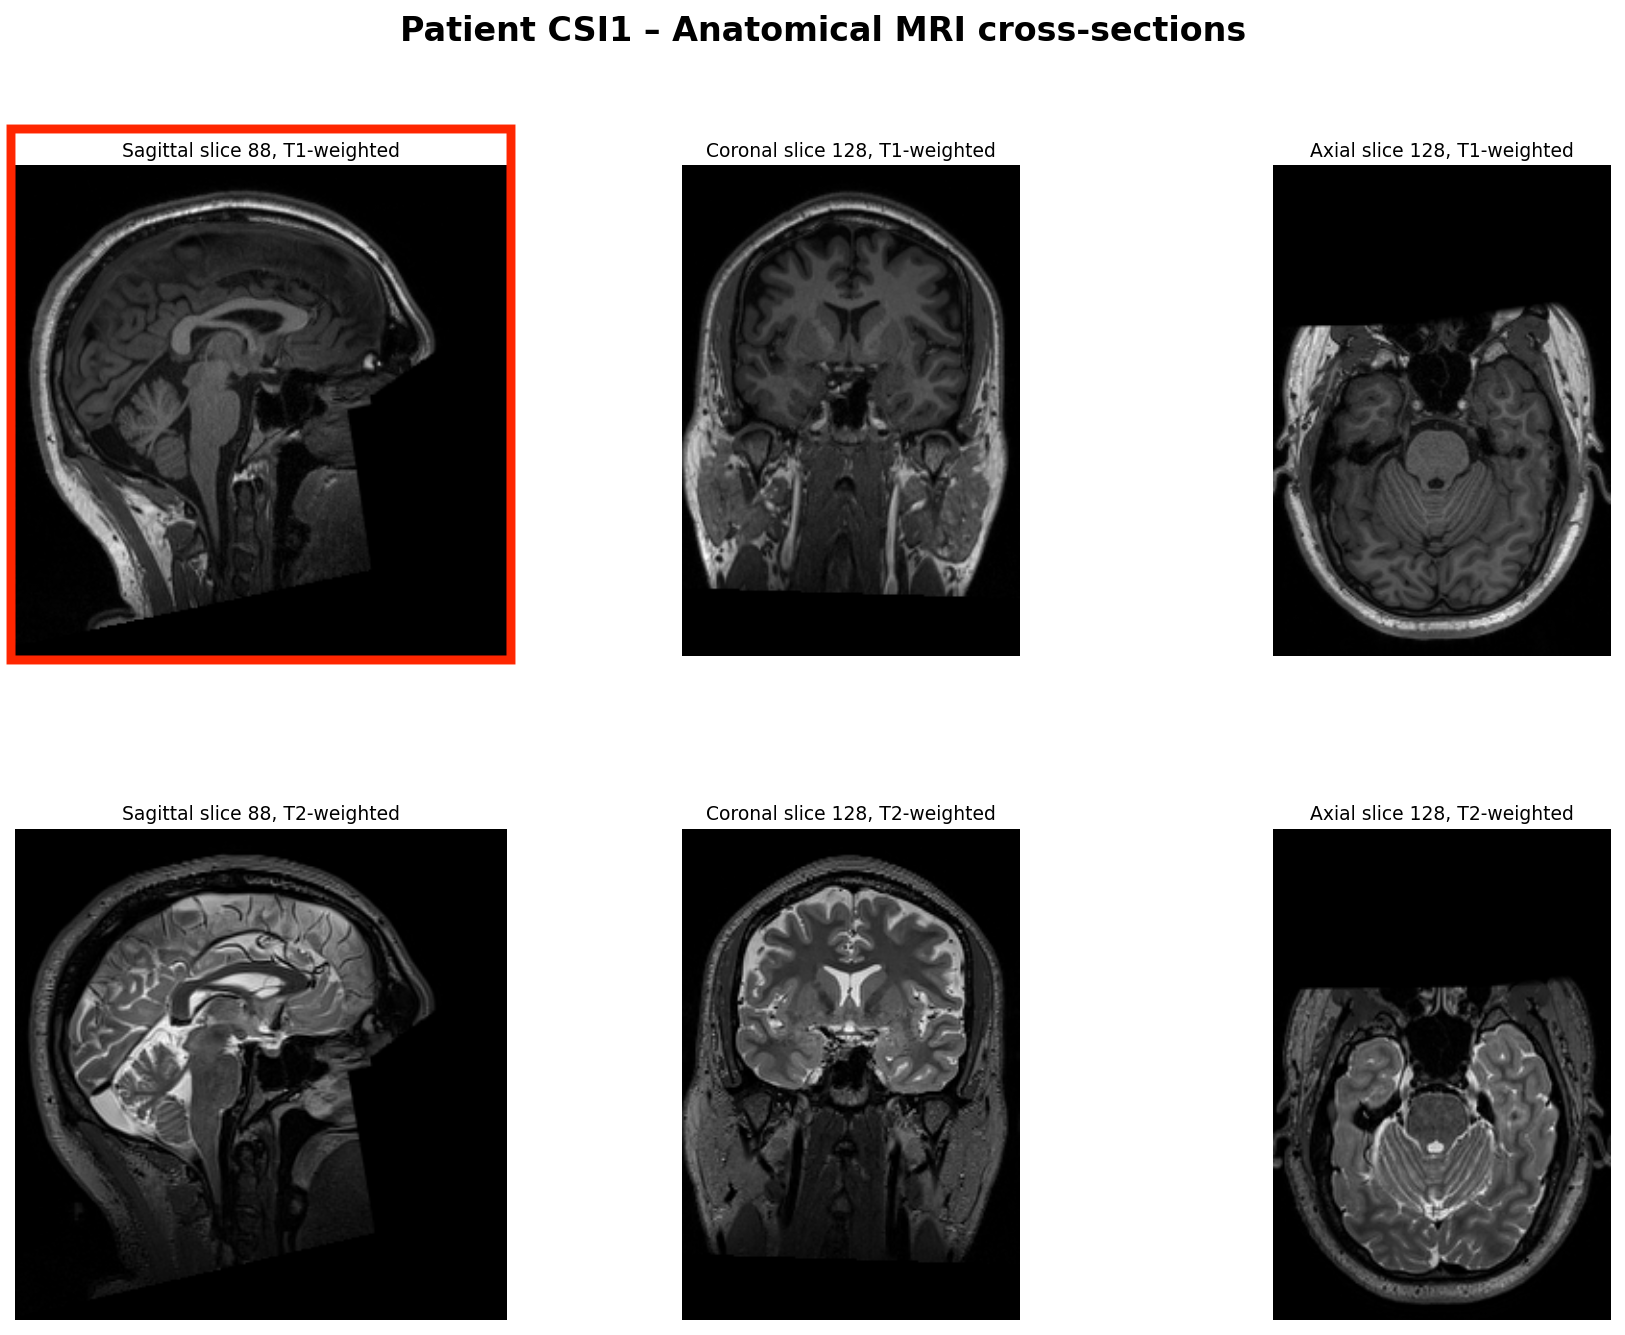
\includegraphics[width=0.9\linewidth]{Results/part1_six_panels.png}
  \caption{Sagittal, coronal, and axial center slices for T1-weighted (top)
  and T2-weighted (bottom) volumes. The guiding image is boxed in red.}
  \label{fig:six_panels}
\end{figure}

\subsection{T1 and T2 Brightness}

From Table~\ref{tab:tissue}, the predicted brightness rankings are:

\textbf{T1-weighted} (shorter $T_1$ $\to$ brighter): WM ($T_1 = 510\,\mathrm{ms}$)
$>$ GM ($760\,\mathrm{ms}$) $>$ CSF ($2650\,\mathrm{ms}$).

\textbf{T2-weighted} (longer $T_2$ $\to$ brighter): CSF ($T_2 = 280\,\mathrm{ms}$)
$>$ GM ($77\,\mathrm{ms}$) $>$ WM ($67\,\mathrm{ms}$).

These predictions are confirmed by visual inspection of
Fig.~\ref{fig:six_panels}, where it can be seen that white matter appears bright and ventricles dark in
the T1 volume, while the CSF-filled ventricles appear bright in the T2
volume.

\subsection{Pulse-Sequence Parameters}

Table~\ref{tab:pulse_seq} lists the relevant timing parameters from the JSON
sidecars.  All times are in seconds, as inferred from their consistency with
the millisecond-scale relaxation values in Table~\ref{tab:tissue}.

\begin{table}[h]
\centering
\caption{Pulse-sequence parameters from JSON sidecars (units: seconds).}
\label{tab:pulse_seq}
\begin{tabular}{lrr}
\toprule
Parameter & T1-weighted & T2-weighted \\
\midrule
Echo Time (TE)        & $\approx 0.003$ & $\approx 0.09$ \\
Repetition Time (TR)  & $\approx 2.5$   & $\approx 8.0$  \\
Inversion Time (TI)   & $\approx 1.83$  & ---            \\
\bottomrule
\end{tabular}
\end{table}

The T1-weighted scan uses a short TE and moderate TR, which favor tissues
with short $T_1$ that recover quickly between pulses and lose little signal
before readout.  The inversion time $TI \approx 0.69 \times T_{1,\mathrm{CSF}}
= 1.83\,\mathrm{s}$ is chosen so that CSF passes through zero magnetization
at the moment of readout, effectively nulling it and sharpening the contrast
between white and grey matter.  The T2-weighted scan uses a long TE and long
TR; the long TR removes T1 bias by allowing all tissues to fully recover, and
the long TE gives transverse magnetization time to decay, so only tissues with
long $T_2$ (like CSF) retain high signal.


% ===========================================================================
\section{Fourier Domain Compression}
\label{sec:fourier}

The Fourier magnitude distribution of the guiding image is sharply
right-skewed, where the bottom 90\% of coefficients by magnitude account for only
a small fraction of the total spectral energy, which is concentrated near the
DC origin (Fig.~\ref{fig:fourier_domain}).  The histogram confirms this
heavily right-skewed distribution, suggesting that aggressive Fourier
truncation might succeed.

\begin{figure}[h]
  \centering
  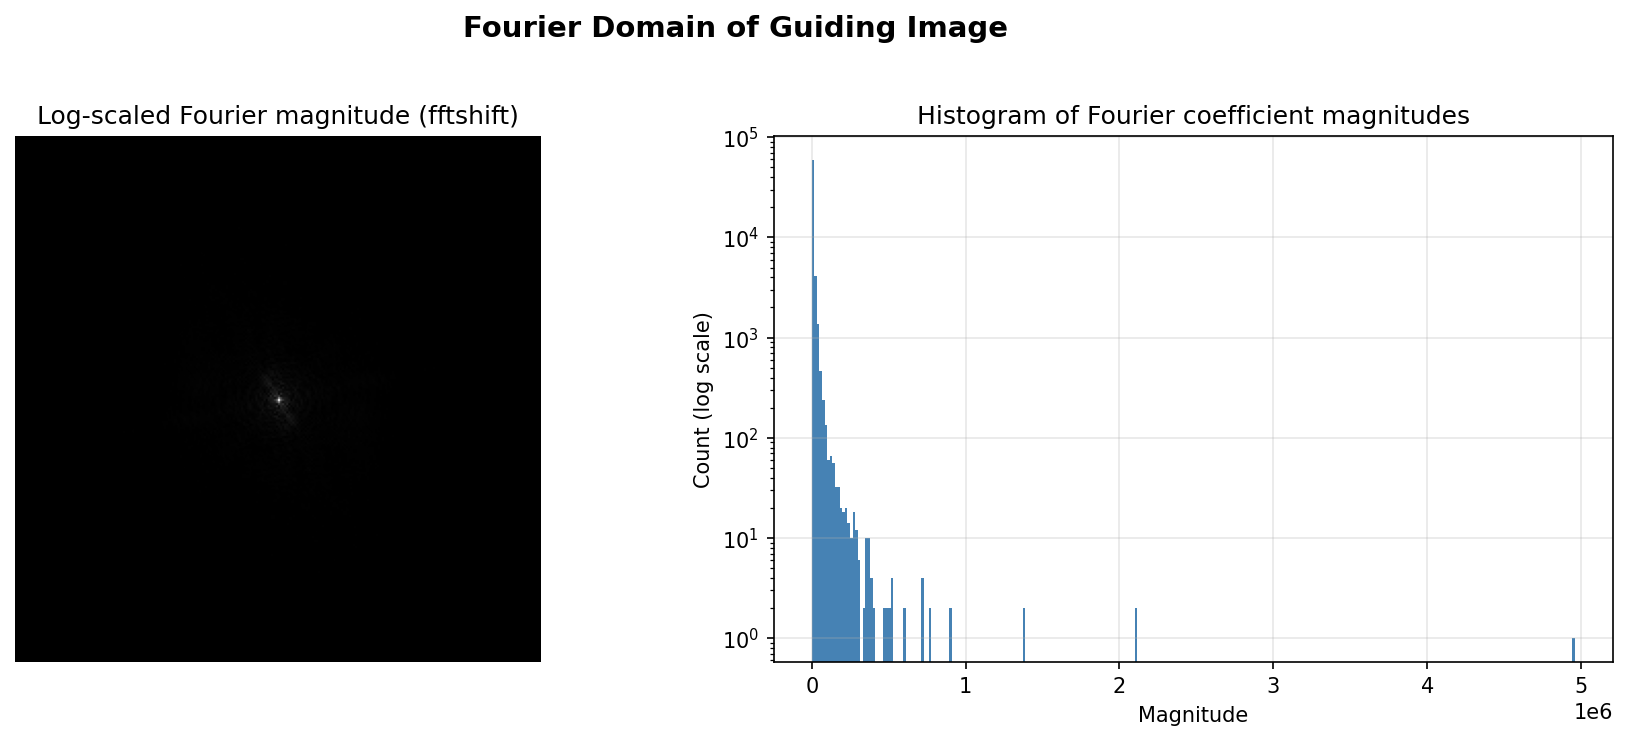
\includegraphics[width=0.9\linewidth]{Results/part3_fourier_domain.png}
  \caption{Log-scaled Fourier magnitude of the guiding image (left) and
  coefficient magnitude histogram (right).}
  \label{fig:fourier_domain}
\end{figure}

Figure~\ref{fig:fourier_compression} and Table~\ref{tab:fourier_error}
summarize reconstruction quality at several compression levels.  Error
concentrates at high-contrast edges and spreads globally as $s$ increases,
reflecting the destruction of phase coherence rather than localized magnitude
loss.

\begin{figure}[h]
  \centering
  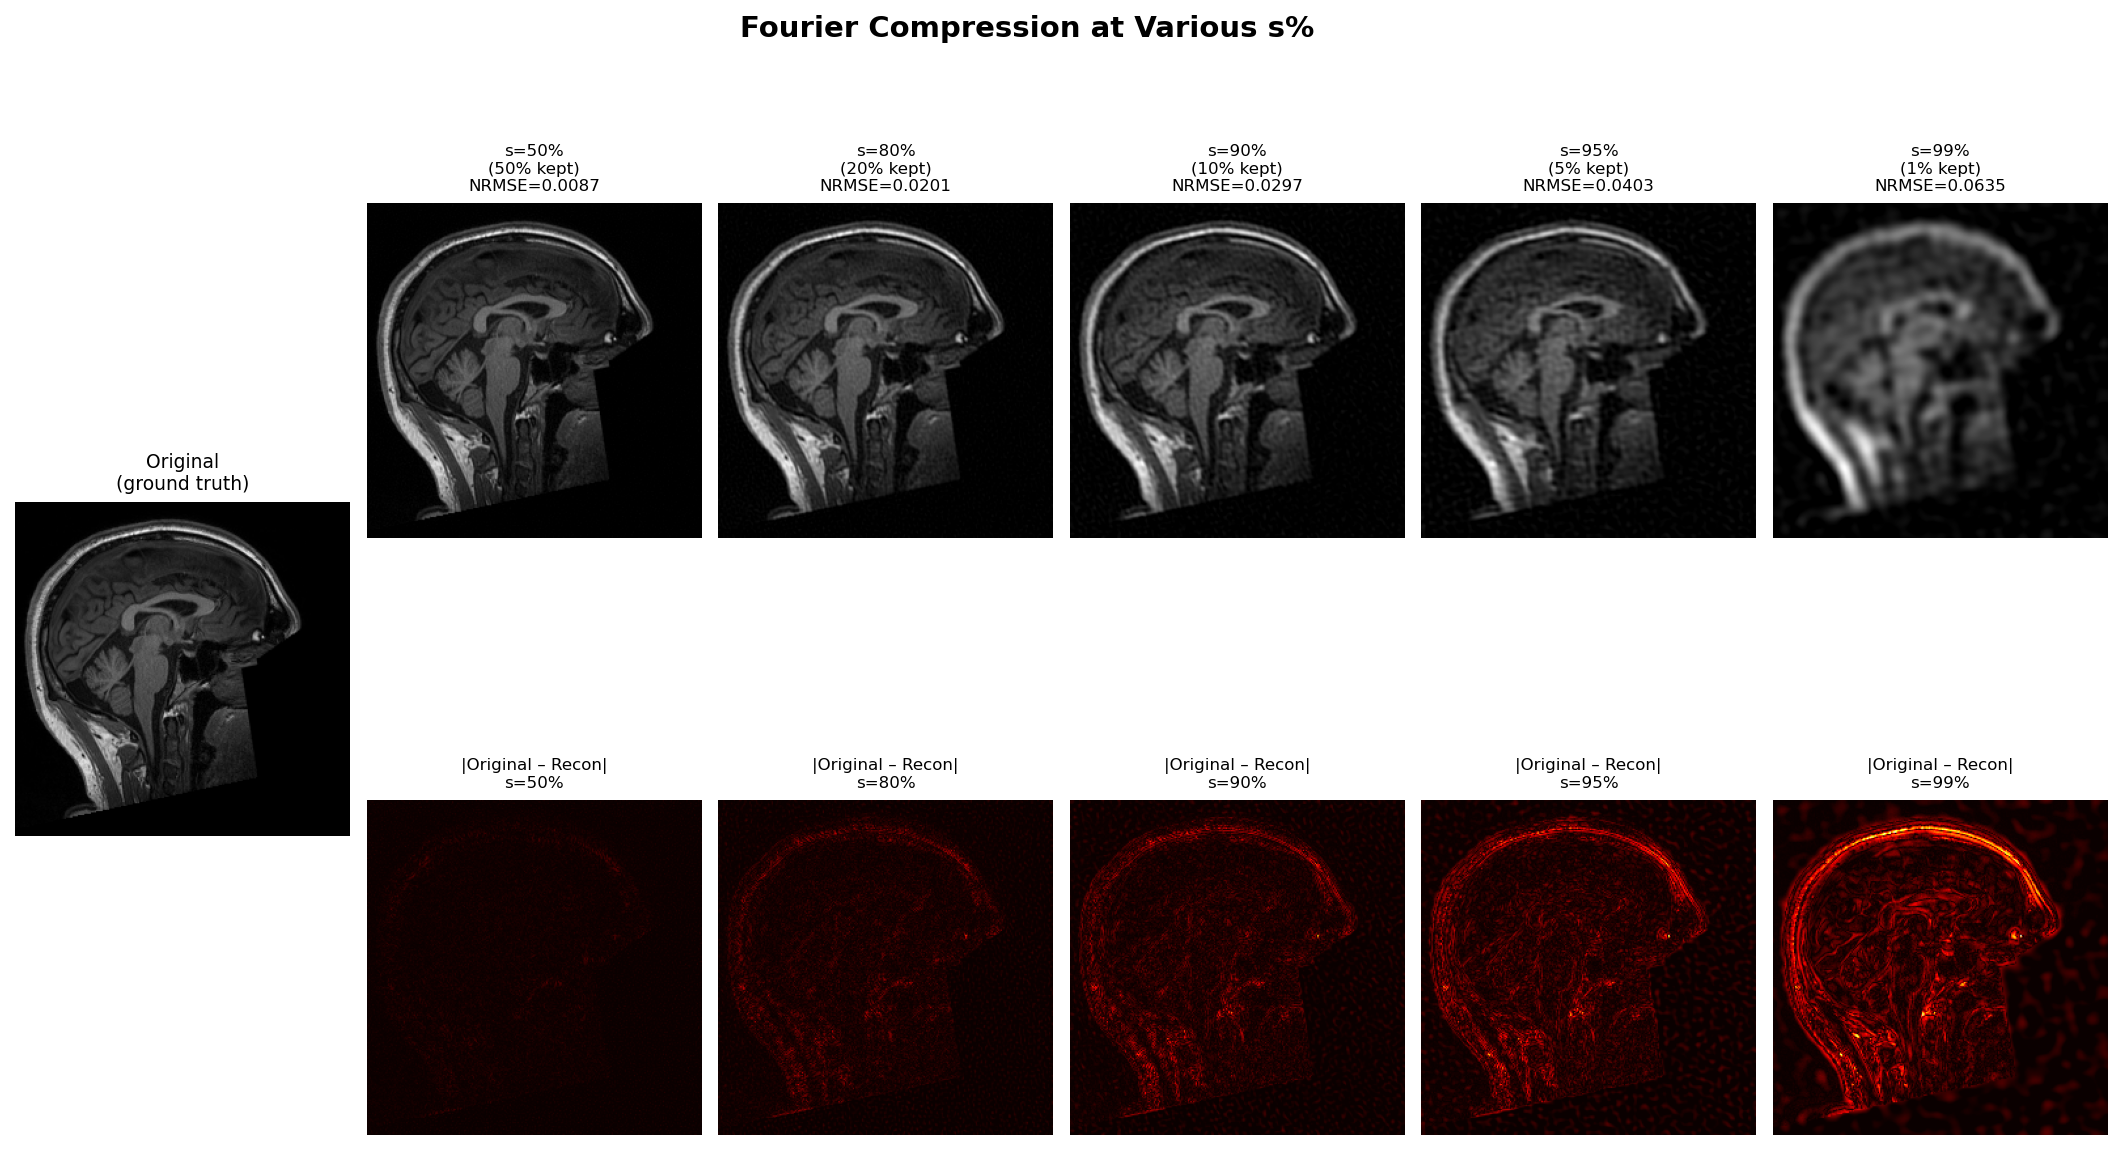
\includegraphics[width=0.9\linewidth]{Results/part3_fourier_compression.png}
  \caption{Fourier compression at $s \in \{50, 80, 90, 95, 99\}\%$.
  Top: reconstructed images. Bottom: absolute error maps on a shared
  color scale.}
  \label{fig:fourier_compression}
\end{figure}

\begin{table}[h]
\centering
\caption{Fourier compression errors on the guiding image.}
\label{tab:fourier_error}
\begin{tabular}{rrr}
\toprule
$s$ (\% zeroed) & \% kept &  NRMSE \\
\midrule
50 & 50 &  0.0087 \\
80 & 20 &  0.0201 \\
90 & 10 &  0.0297 \\
95 & 5  &  0.0403 \\
99 & 1  &  0.0635 \\
\bottomrule
\end{tabular}
\end{table}

Despite numerically small NRMSE values, the reconstructed images at
$s \geq 90\%$ exhibit severe blur and visual artifacts. To explain this, we must remember that the small-magnitude Fourier coefficients encode
critical phase information.  Phase determines the spatial arrangement of
image features and is non-redundant. When we null a coefficient at frequency
$(u,v)$, we perturb every spatial location through the inverse transform.
Consequently, even when the discarded magnitudes are small, the destruction
of global phase coherence produces spatially widespread artifacts that are
perceptually salient.

Thus, although the Fourier magnitude distribution is sparse,
the Fourier domain is unsuitable for image compression because phase
information cannot be selectively discarded.  This motivates the use of
localized wavelet bases, which achieve simultaneous spatial and frequency
localization.


% ===========================================================================
\section{Wavelet-Domain Analysis}
\label{sec:wavelet}

\subsection{Basis Functions}
To visualize what each wavelet "looks like," a single coefficient was set
to 1 in the level-1 detail subband and the inverse DWT was applied,
producing the spatial pattern that one coefficient contributes to the image.
The Fourier magnitude of this pattern then shows which frequencies that
coefficient captures (Fig.~\ref{fig:basis_elements}).

\begin{figure}[h]
  \centering
  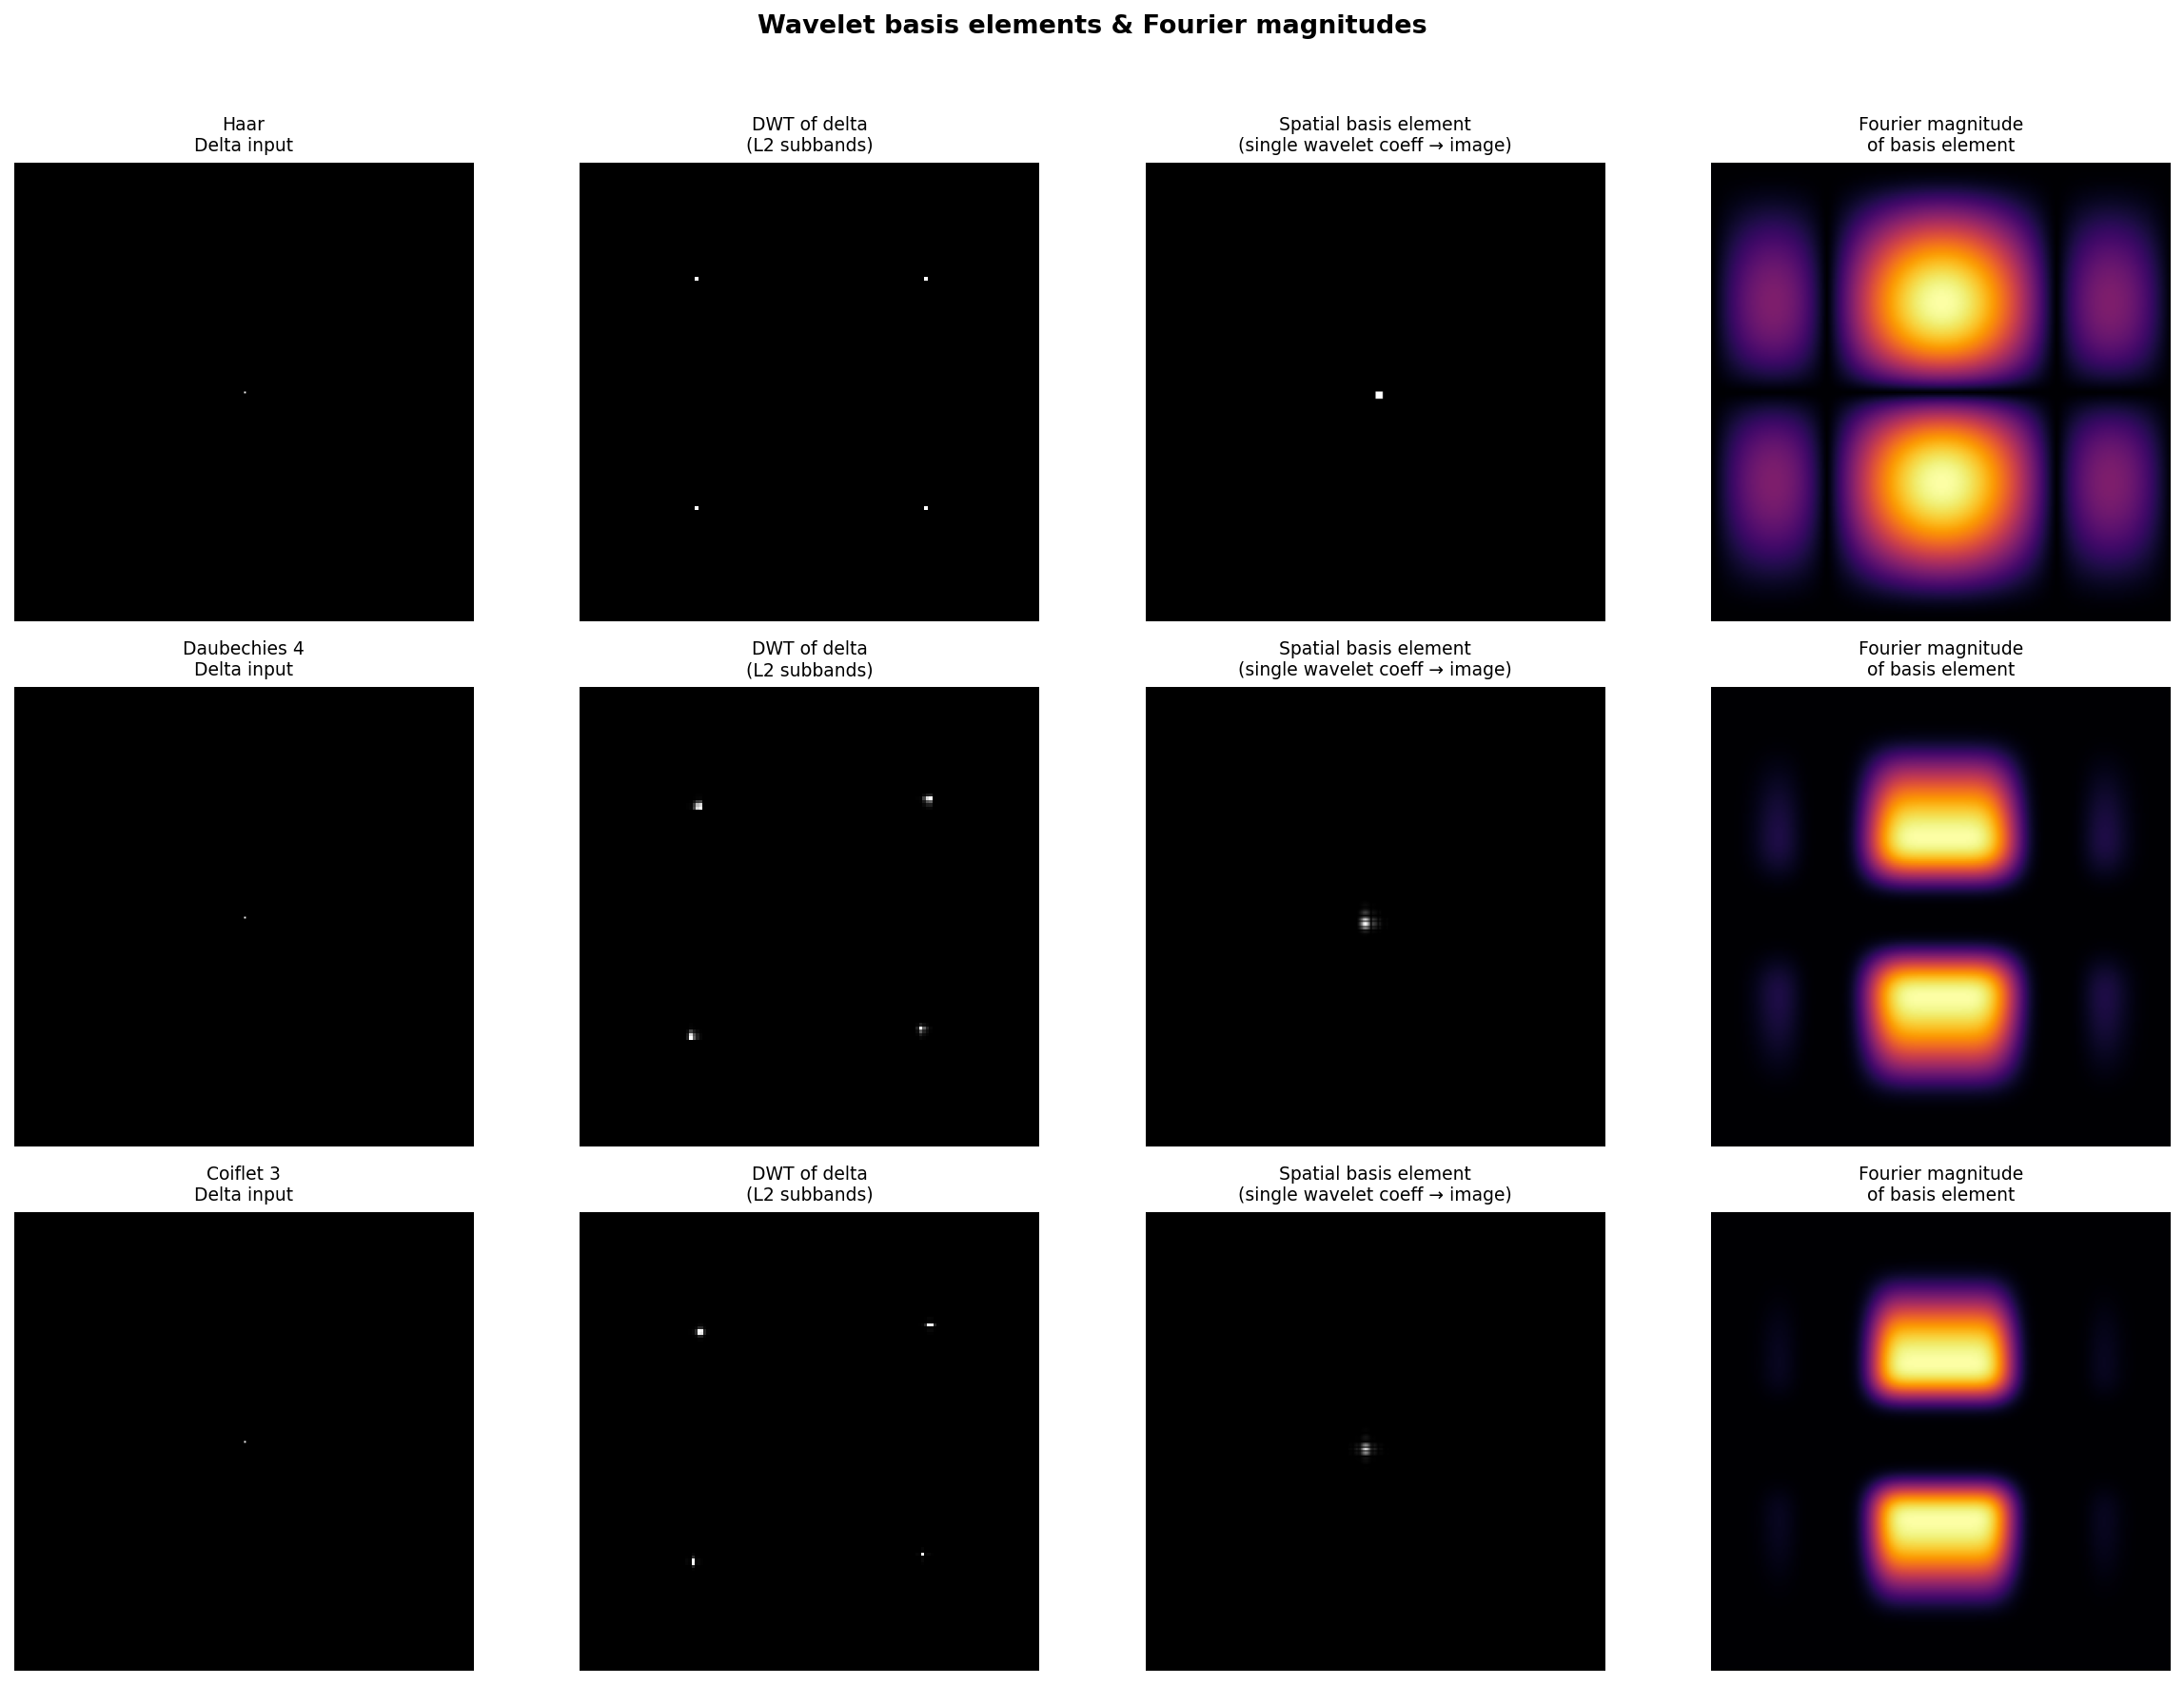
\includegraphics[width=0.9\linewidth]{Results/part4B_basis_elements.png}
  \caption{Wavelet basis element analysis for Haar (top), Daubechies~4
  (middle), and Coiflet~3 (bottom). Columns: delta input, DWT of delta,
  spatial pattern of a single coefficient, and its Fourier magnitude.}
  \label{fig:basis_elements}
\end{figure}

Haar produces a small box-shaped spatial pattern whose Fourier magnitude
spreads broadly across four lobes, meaning each coefficient mixes many
frequencies.  Daubechies~4 is smoother and its frequency response is more
contained.  Coiflet~3 produces the most compact spatial pattern and the
tightest frequency response of the three, meaning its coefficients capture
a narrower, better-defined range of frequencies.  This improving
localization with each basis directly explains the sparsity ordering seen in the histograms (Fig. ~\ref{fig:histograms}).

Figure~\ref{fig:wavelet_functions} shows the 1D wavelet shapes.  Haar is
a simple step function, which is why it
has poor frequency selectivity.  Daubechies~4 is smooth but asymmetric.
Coiflet~3 is both smooth and nearly symmetric, a consequence of its six
vanishing moments, and this balance between space and frequency is what
makes it the best compressor of the three.

\begin{figure}[h]
  \centering
  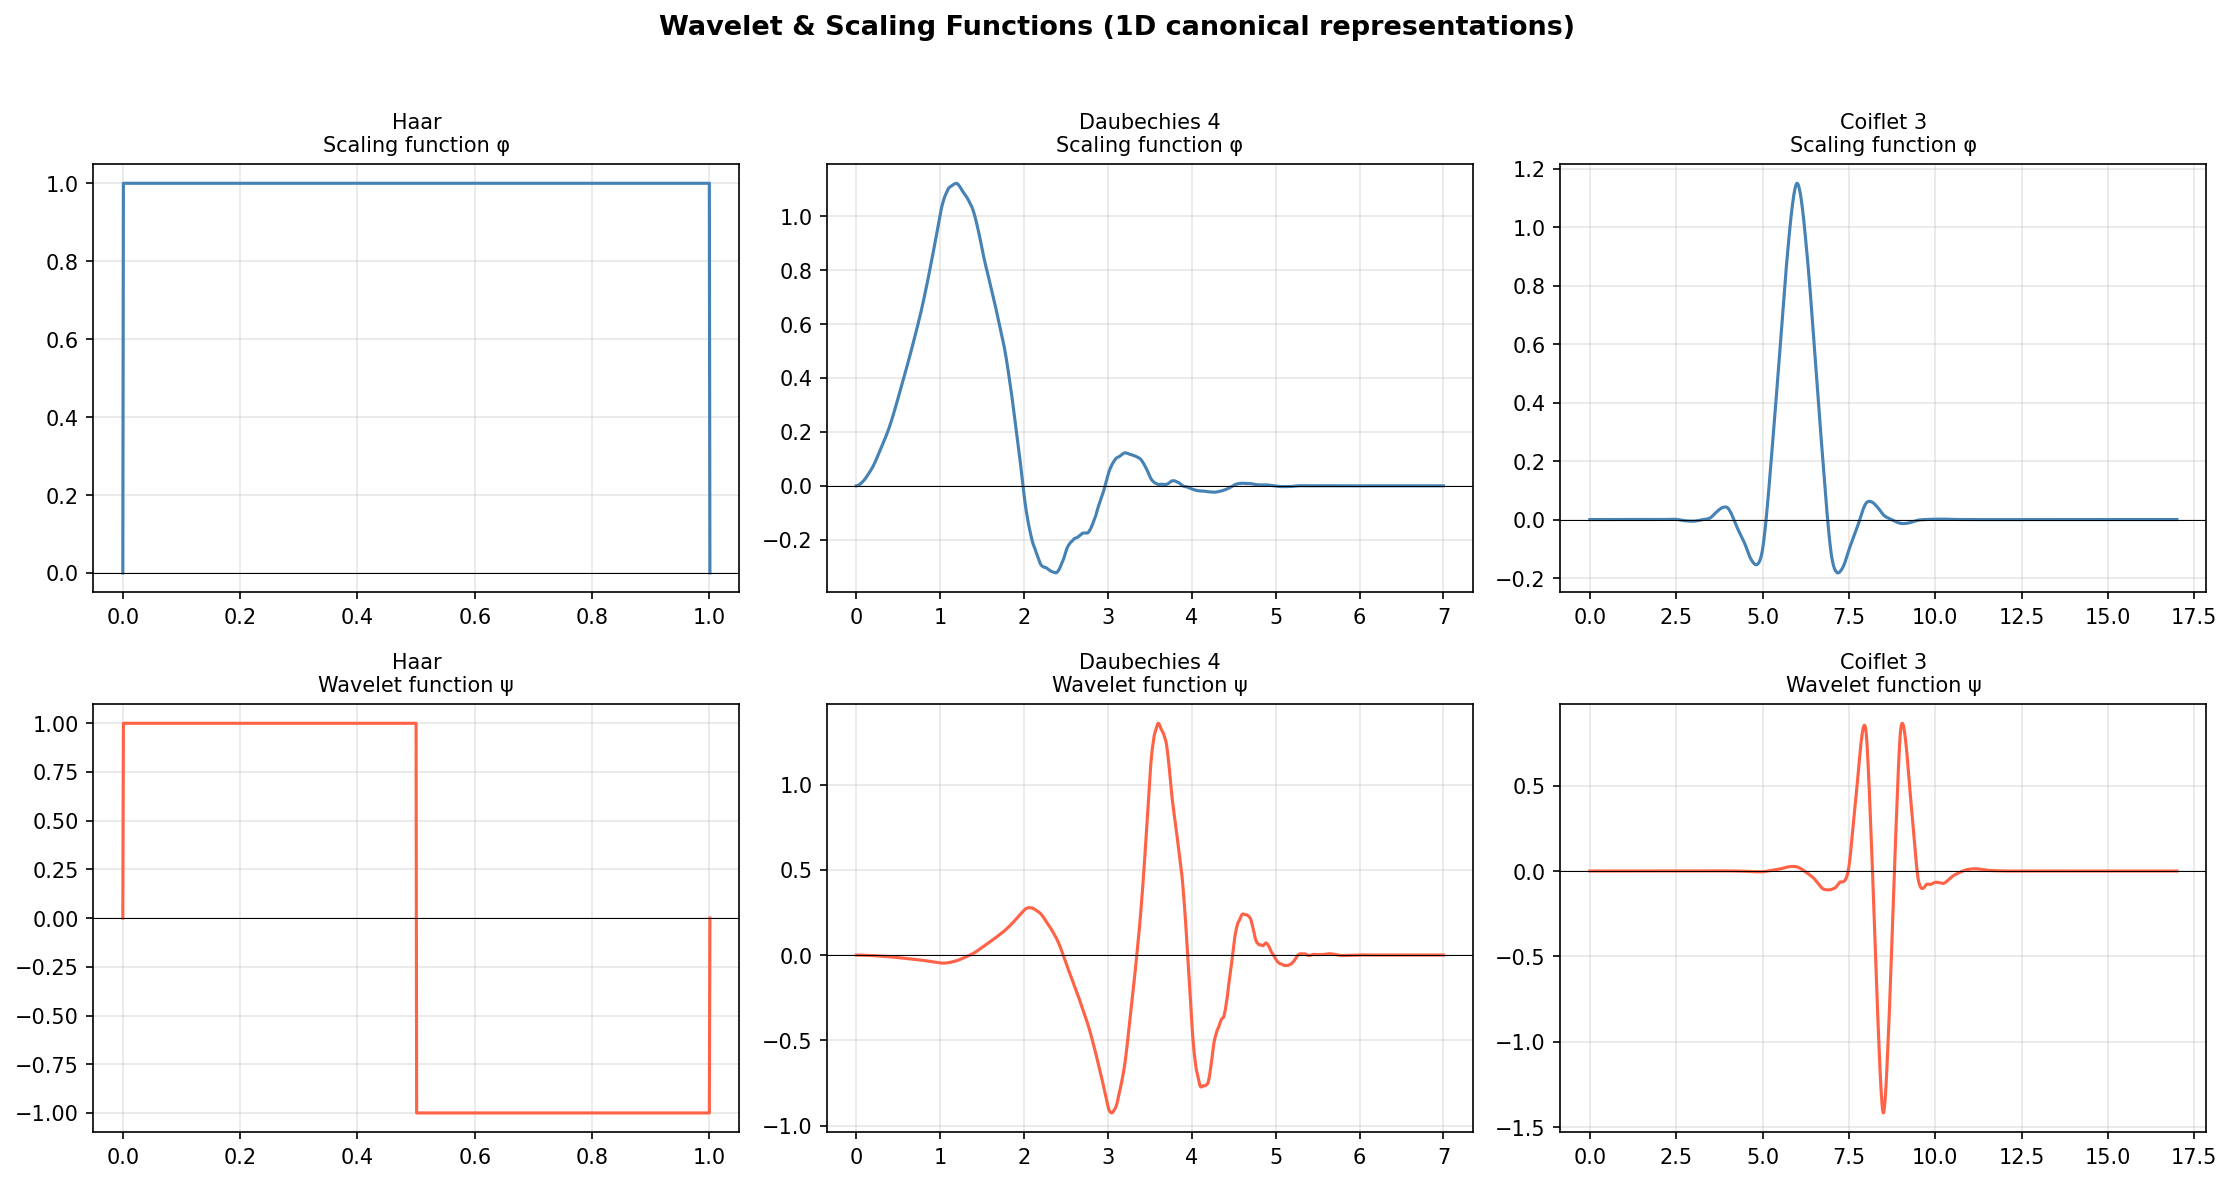
\includegraphics[width=0.9\linewidth]{Results/part4B_wavelet_functions.png}
  \caption{1D scaling functions $\phi$ (top) and wavelet functions $\psi$
  (bottom) for Haar, Daubechies~4, and Coiflet~3.}
  \label{fig:wavelet_functions}
\end{figure}

\subsection{Decompositions of the Guiding Image}
Figures~\ref{fig:dwt_haar}--\ref{fig:dwt_coif3} show the 2-level DWT of the guiding image for all three bases.  In each case the approximation subband captures the coarse anatomical structure, while
the six detail subbands respond primarily at tissue boundaries and edges,
at two scales and three orientations (horizontal, vertical, diagonal).
Haar detail subbands show blockier, less localized responses,
while Coiflet~3 produces sharper, more spatially precise edge responses,
consistent with its better frequency localization. 

\begin{figure}[h]
  \centering
  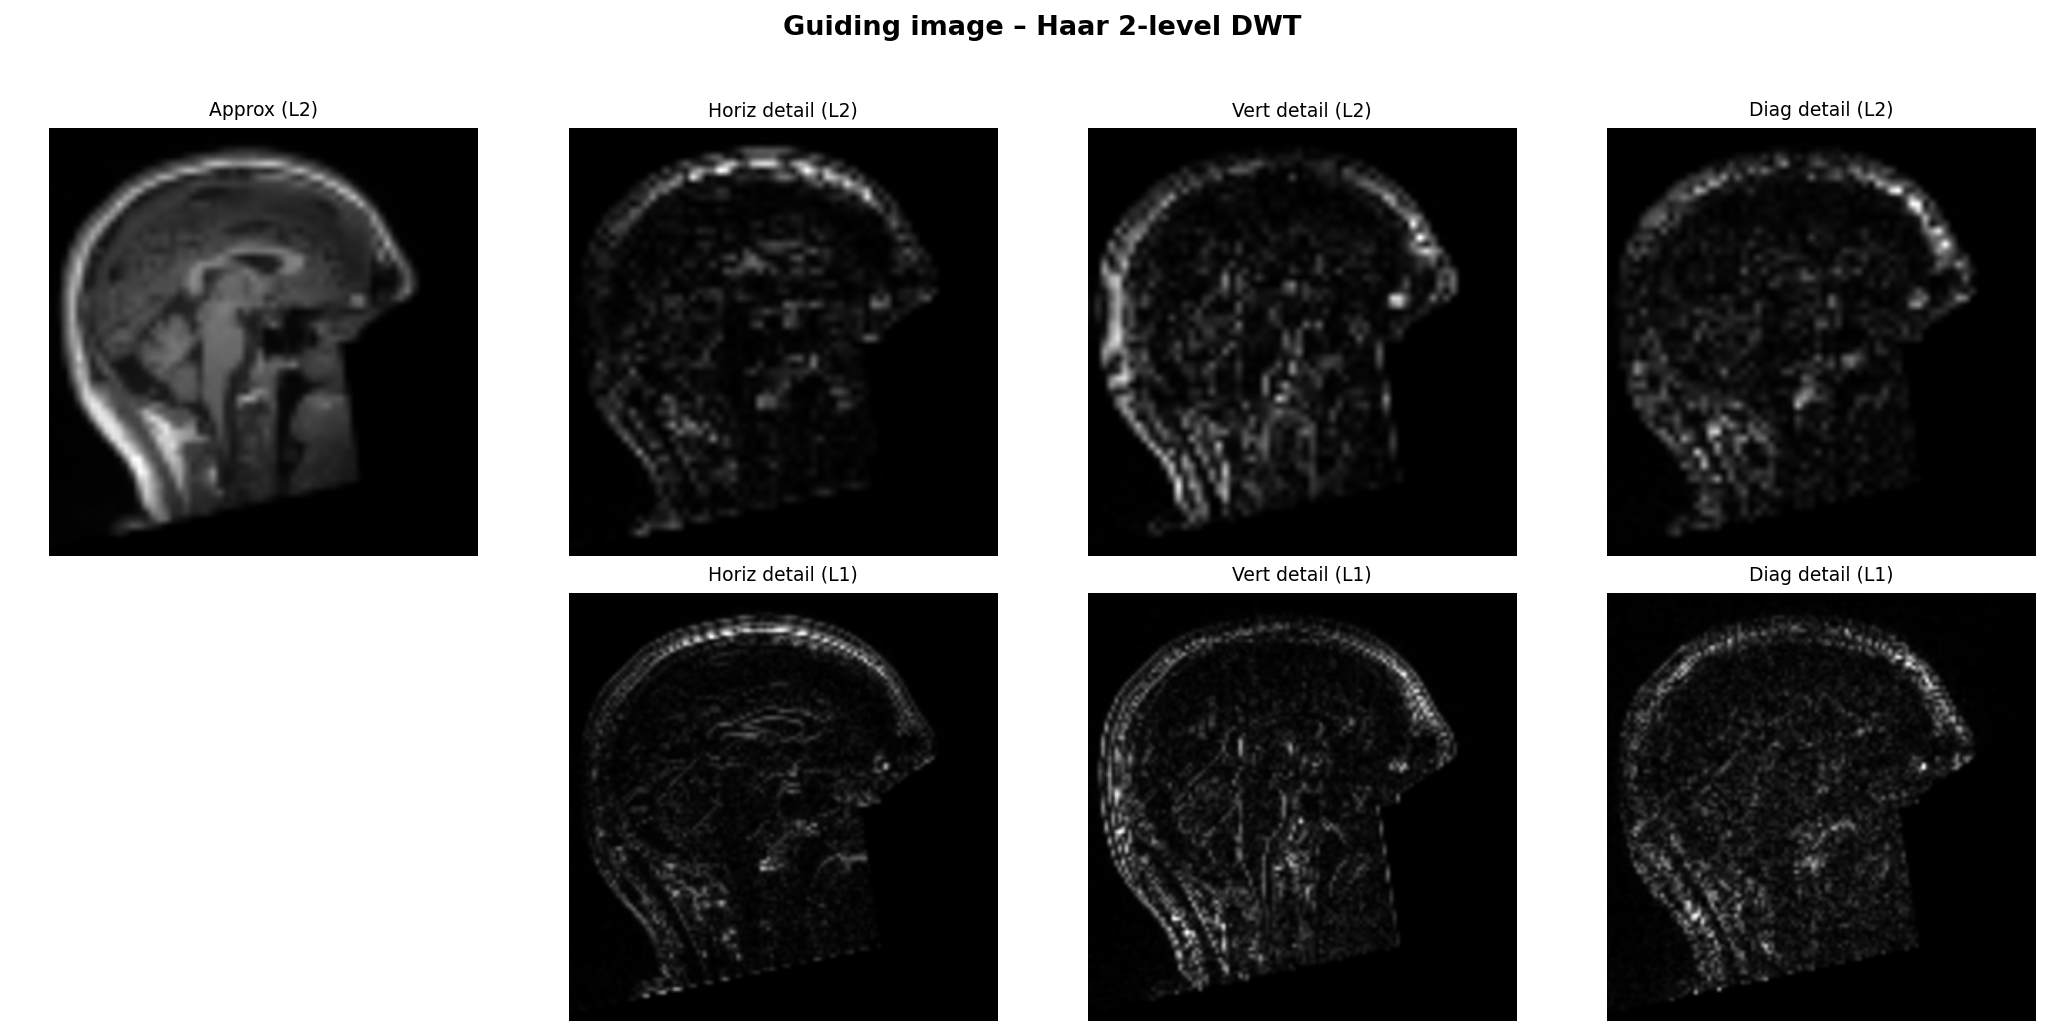
\includegraphics[width=0.9\linewidth]{Results/part4C_guiding_haar.png}
  \caption{Two-level Haar decomposition of the guiding image.}
  \label{fig:dwt_haar}
\end{figure}

\begin{figure}[h]
  \centering
  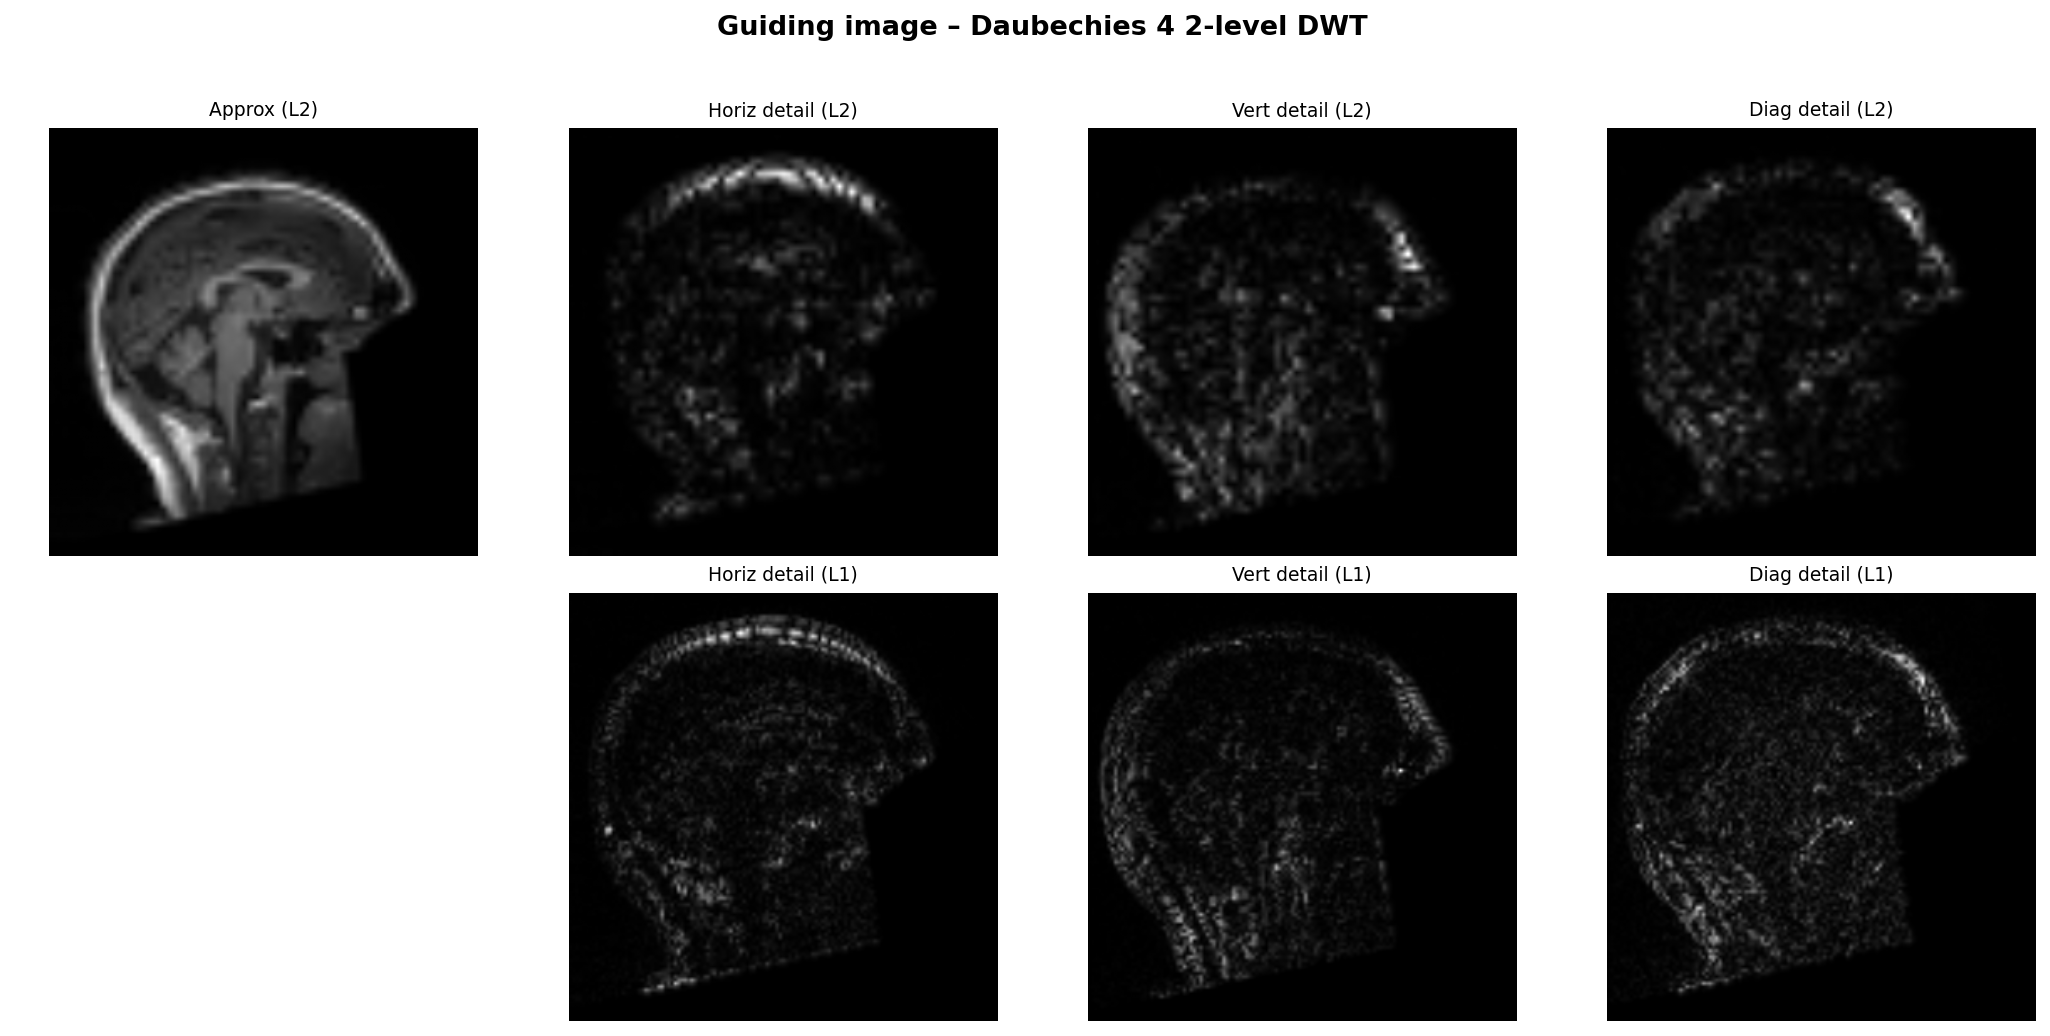
\includegraphics[width=0.9\linewidth]{Results/part4C_guiding_db4.png}
  \caption{Two-level Daubechies~4 decomposition of the guiding image.}
  \label{fig:dwt_db4}
\end{figure}

\begin{figure}[h]
  \centering
  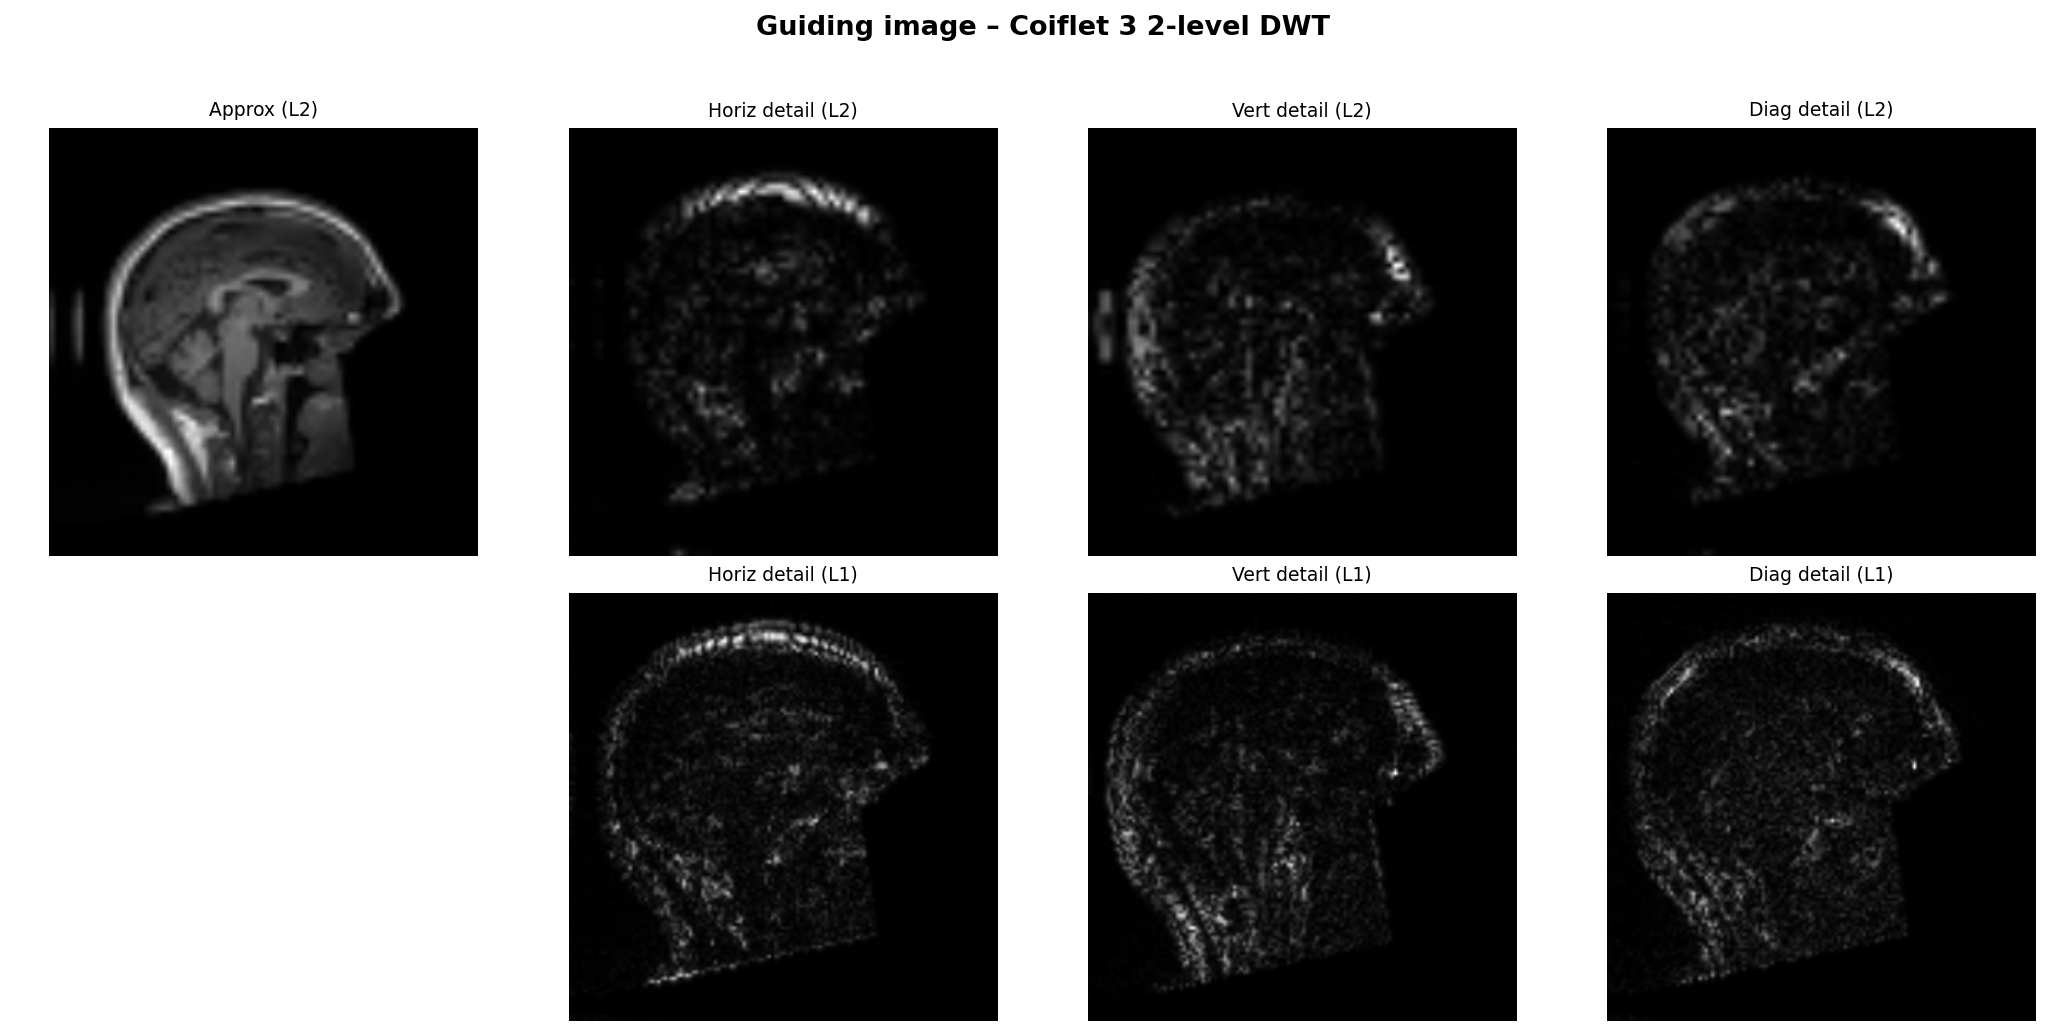
\includegraphics[width=0.9\linewidth]{Results/part4C_guiding_coif3.png}
  \caption{Two-level Coiflet~3 decomposition of the guiding image.}
  \label{fig:dwt_coif3}
\end{figure}

\subsection{Coefficient Histograms and Sparsity Quantification}

Figure~\ref{fig:histograms} shows histograms of pooled DWT coefficients for
all three bases at decomposition levels 1, 2, and 3.  All distributions are
sharply peaked at zero with heavy tails (indicating sparsity).

\begin{figure}[h]
  \centering
  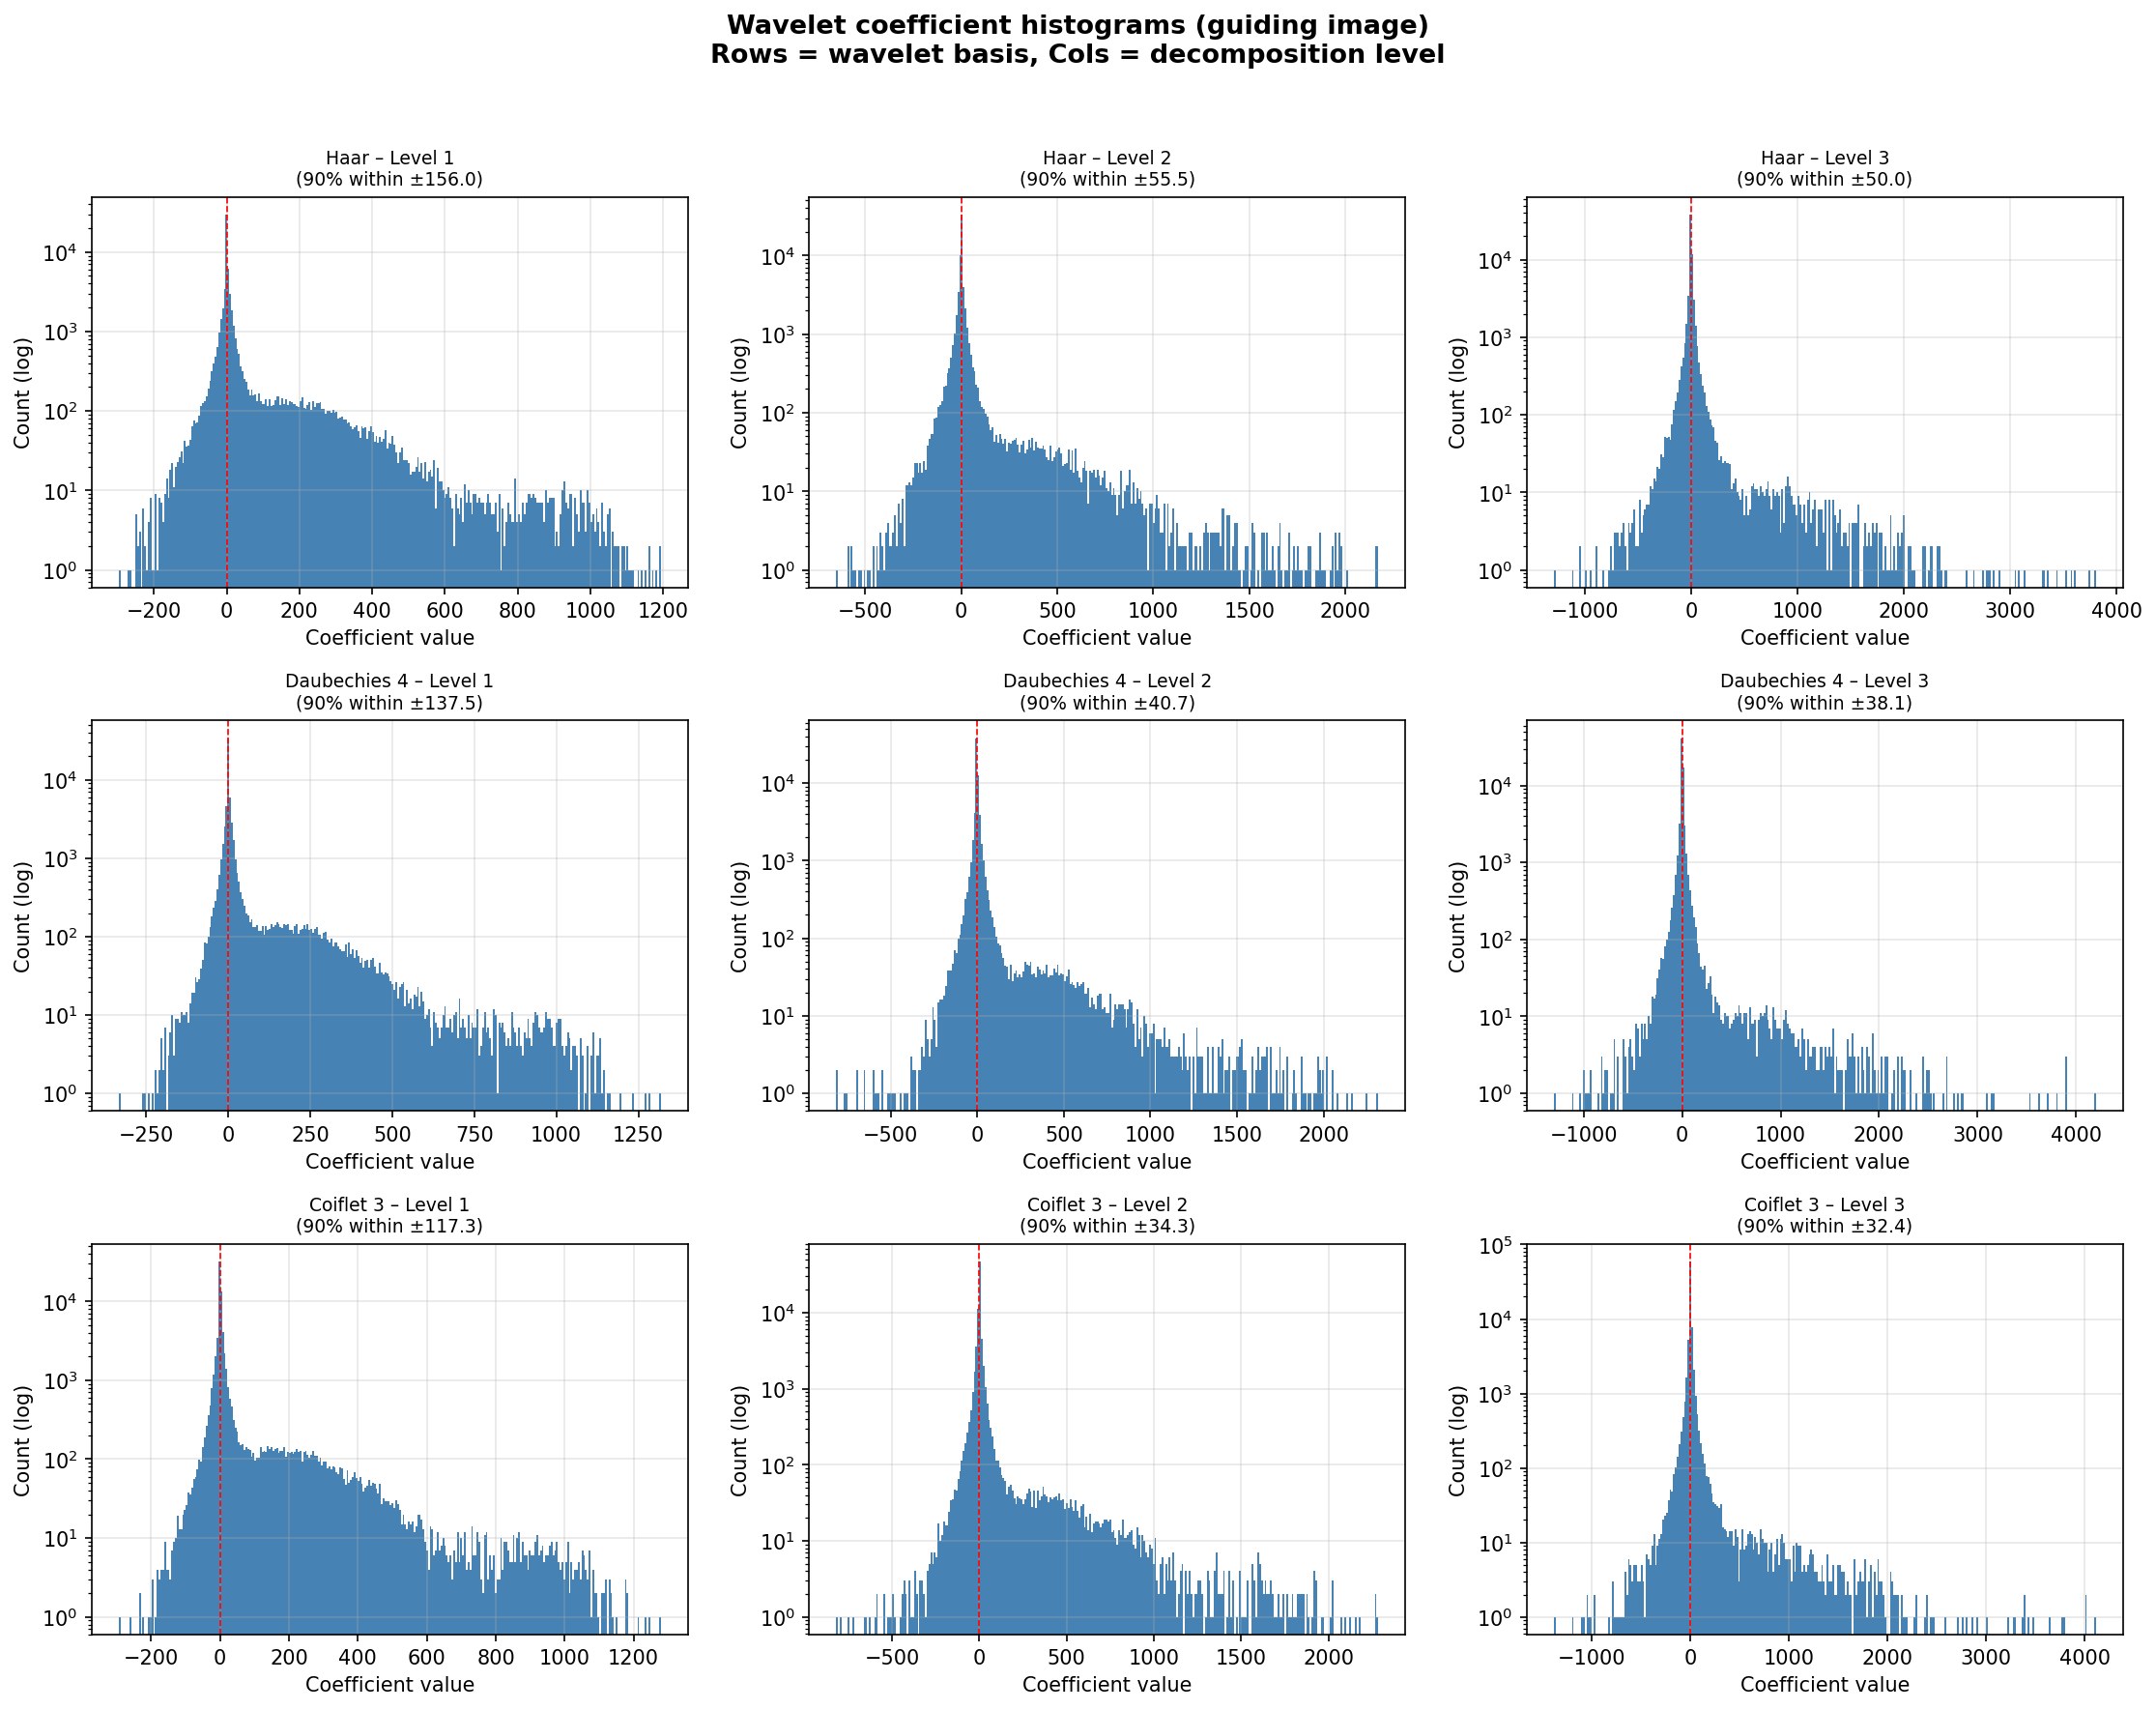
\includegraphics[width=0.9\linewidth]{Results/part4D_histograms.png}
  \caption{Wavelet coefficient histograms for all three bases at levels 1--3
  ($3\times3$ grid, log-scale). Red dashed line marks zero.}
  \label{fig:histograms}
\end{figure}

Table~\ref{tab:sparsity} reports the 90th-percentile absolute coefficient
value as a proxy for sparsity; 90\% of coefficients lie within the interval
$[-\text{threshold},+\text{threshold}]$.

\begin{table}[h]
\centering
\caption{90th-percentile coefficient magnitude (lower = sparser).}
\label{tab:sparsity}
\begin{tabular}{lrr}
\toprule
Basis & Level 2 & Level 3 \\
\midrule
Haar          & $\pm55.5$ & $\pm50.0$ \\
Daubechies~4  & $\pm40.0$ & $\pm37.4$ \\
Coiflet~3     & $\pm34.5$ & $\pm32.6$ \\
\bottomrule
\end{tabular}
\end{table}

Coiflet~3 is the sparsest at every level and visually looks to be the "tightest" around the origin in its histogram; thus, we will utilize Coiflet~3 as the main wavelet domain for following compression and CS analysis.

\subsection{Best Basis Reconstruction}

Figure~\ref{fig:best_basis} shows the result of zeroing the lowest 10\% of Coiflet~3 coefficients by magnitude (level=2) and reconstructing.
The error map is visually indistinguishable from black and the reported
NRMSE is 0.0000.  This is not simply because 10\% is a mild threshold, but rather it is because 19.5\% of Coiflet~3 coefficients are already
identically zero, so the 10th-percentile cutoff falls at exactly zero
and no coefficients are actually discarded.  The residual error of
$\mathrm{MSE} = 4.3\times10^{-27}$ is attributable entirely to
floating-point rounding accumulated over the forward and inverse DWT,
not to any information loss.  This confirms that Coiflet~3 produces a
naturally sparse representation of this MRI image with no thresholding
required.

\begin{figure}[h]
  \centering
  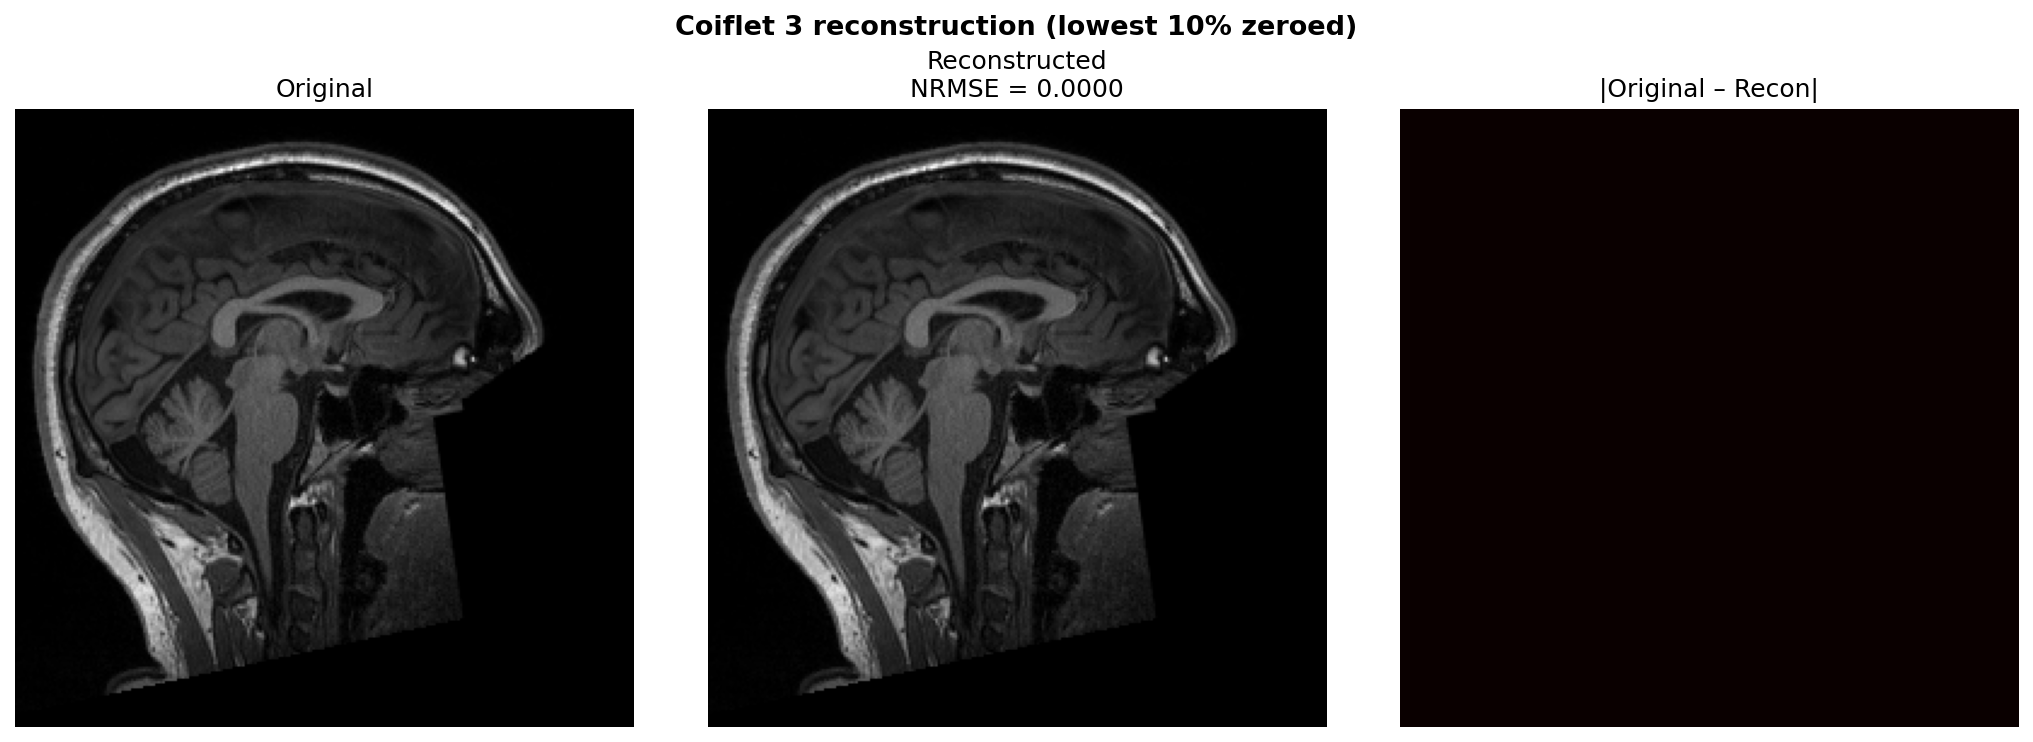
\includegraphics[width=0.9\linewidth]{Results/part4E_best_basis_recon.png}
  \caption{Coiflet~3 reconstruction with the lowest 10\% of coefficients
  zeroed (level=2).}
  \label{fig:best_basis}
\end{figure}

% ===========================================================================
\section{Quantitative Sparsity Analysis}
\label{sec:sparsity}

\subsection{NRMSE as a Function of Compression Ratio}

Figure~\ref{fig:nrmse_vs_s} plots NRMSE against the fraction of zeroed
coefficients $s$ for all three bases.  The Coiflet~3 and Daubechies~4 curves
remain below the 10\% NRMSE threshold for the entire range
$s \in [0, 99]\%$.  The Haar basis first exceeds 10\% NRMSE only at
$s=99\%$.  Though not shown, at level~3, even Haar remains below the threshold at all tested
compression levels.

\begin{figure}[h]
  \centering
  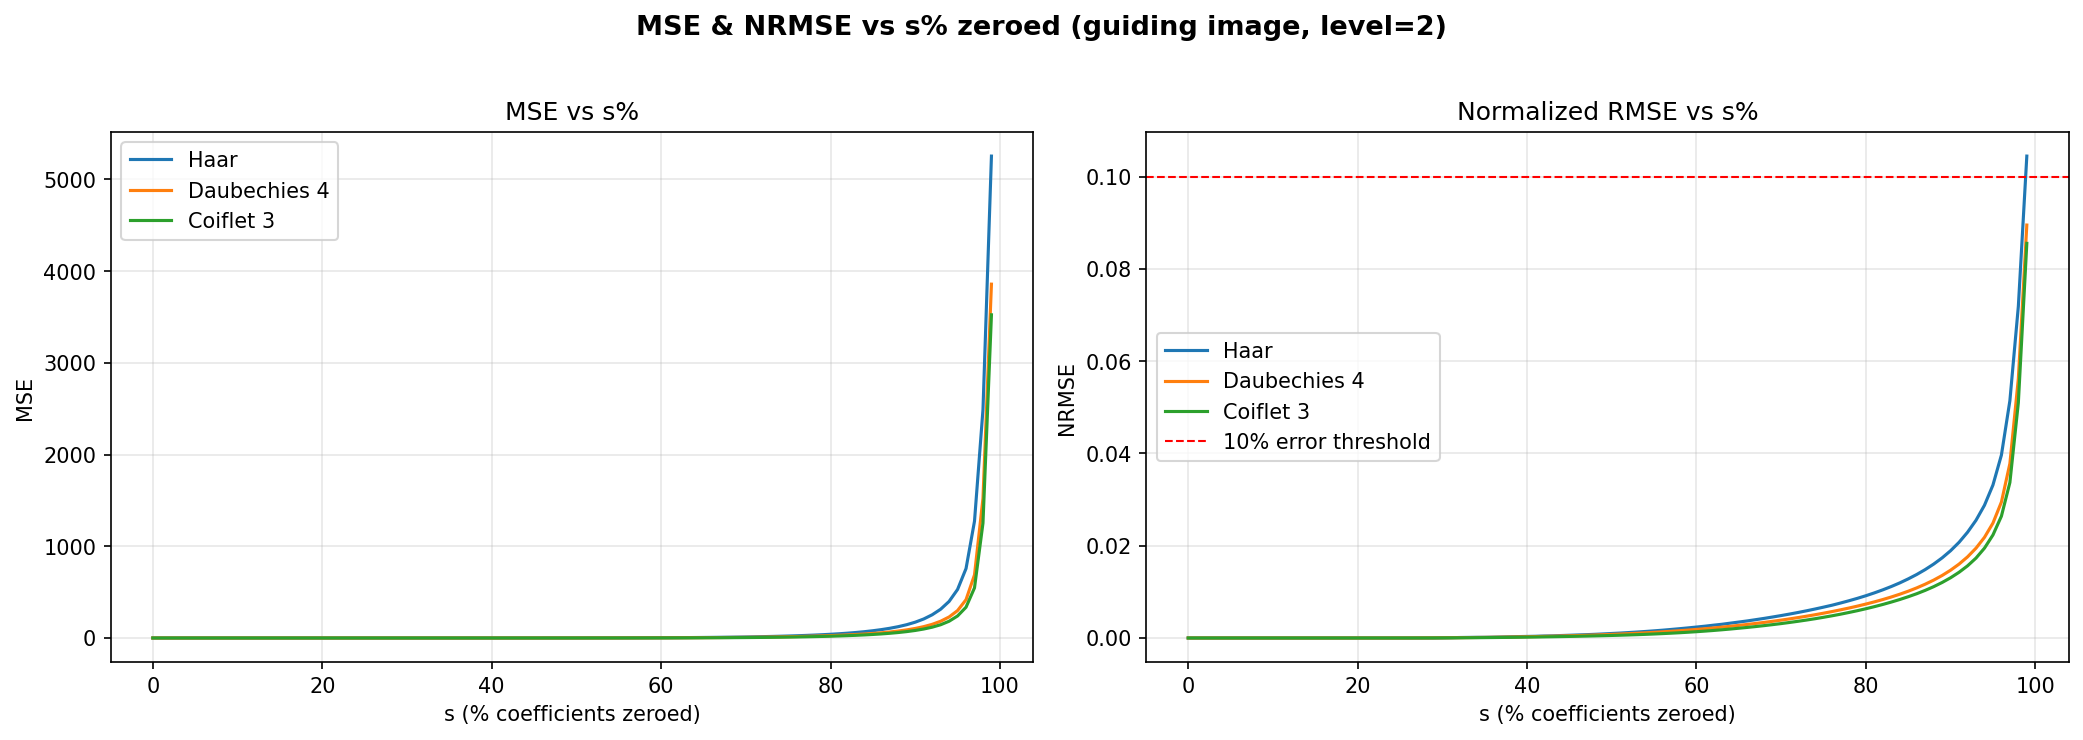
\includegraphics[width=0.9\linewidth]{Results/part5A_mse_vs_s.png}
  \caption{NRMSE vs.\ $s\%$ zeroed for all three bases at level~2.
  Red dashed line: 10\% threshold.}
  \label{fig:nrmse_vs_s}
\end{figure}

Figures~\ref{fig:recons_coif3}--\ref{fig:recons_haar} show reconstructed
images and error maps at $s \in \{50, 80, 90, 95\}\%$ for each basis.
At $s=50\%$ all three bases produce visually clean reconstructions with
NRMSE $= 0.001$.  Degradation begins to appear in the error maps around
$s=80\%$. Interestingly, the degradation is spread uniformly across the brain rather than concentrating
at edges, in contrast to the edge-localized error seen in Fourier compression and reconstruction.

\begin{figure}[h]
  \centering
  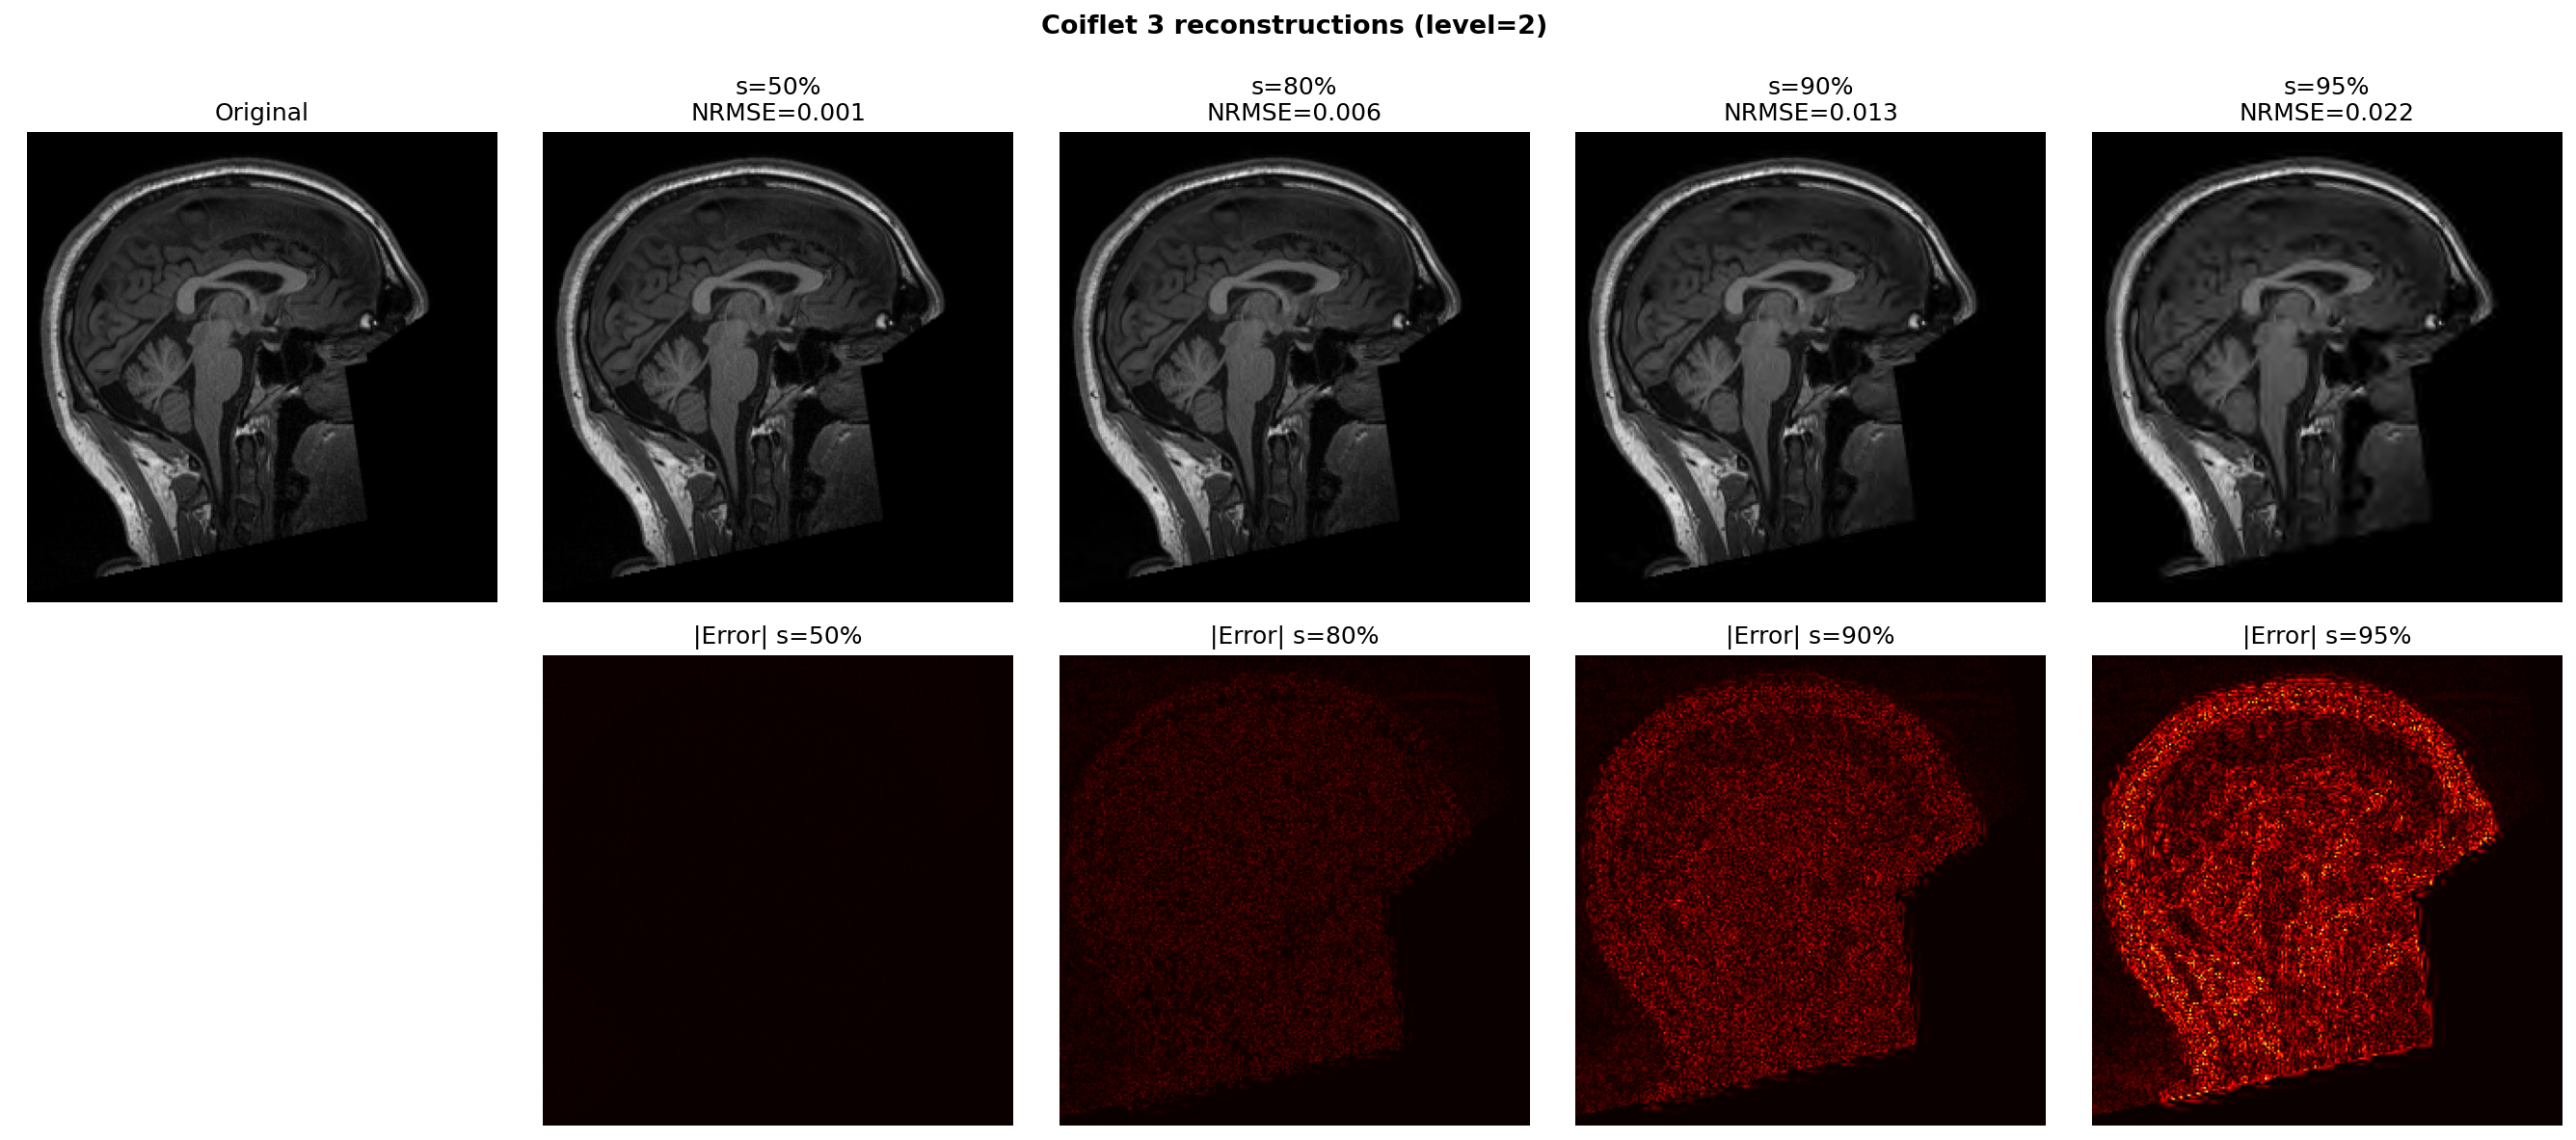
\includegraphics[width=0.9\linewidth]{Results/part5C_recons_coif3.png}
  \caption{Coiflet~3 reconstructions at $s \in \{50, 80, 90, 95\}\%$
  (level=2). Top: reconstructed images. Bottom: absolute error maps.}
  \label{fig:recons_coif3}
\end{figure}

\begin{figure}[h]
  \centering
  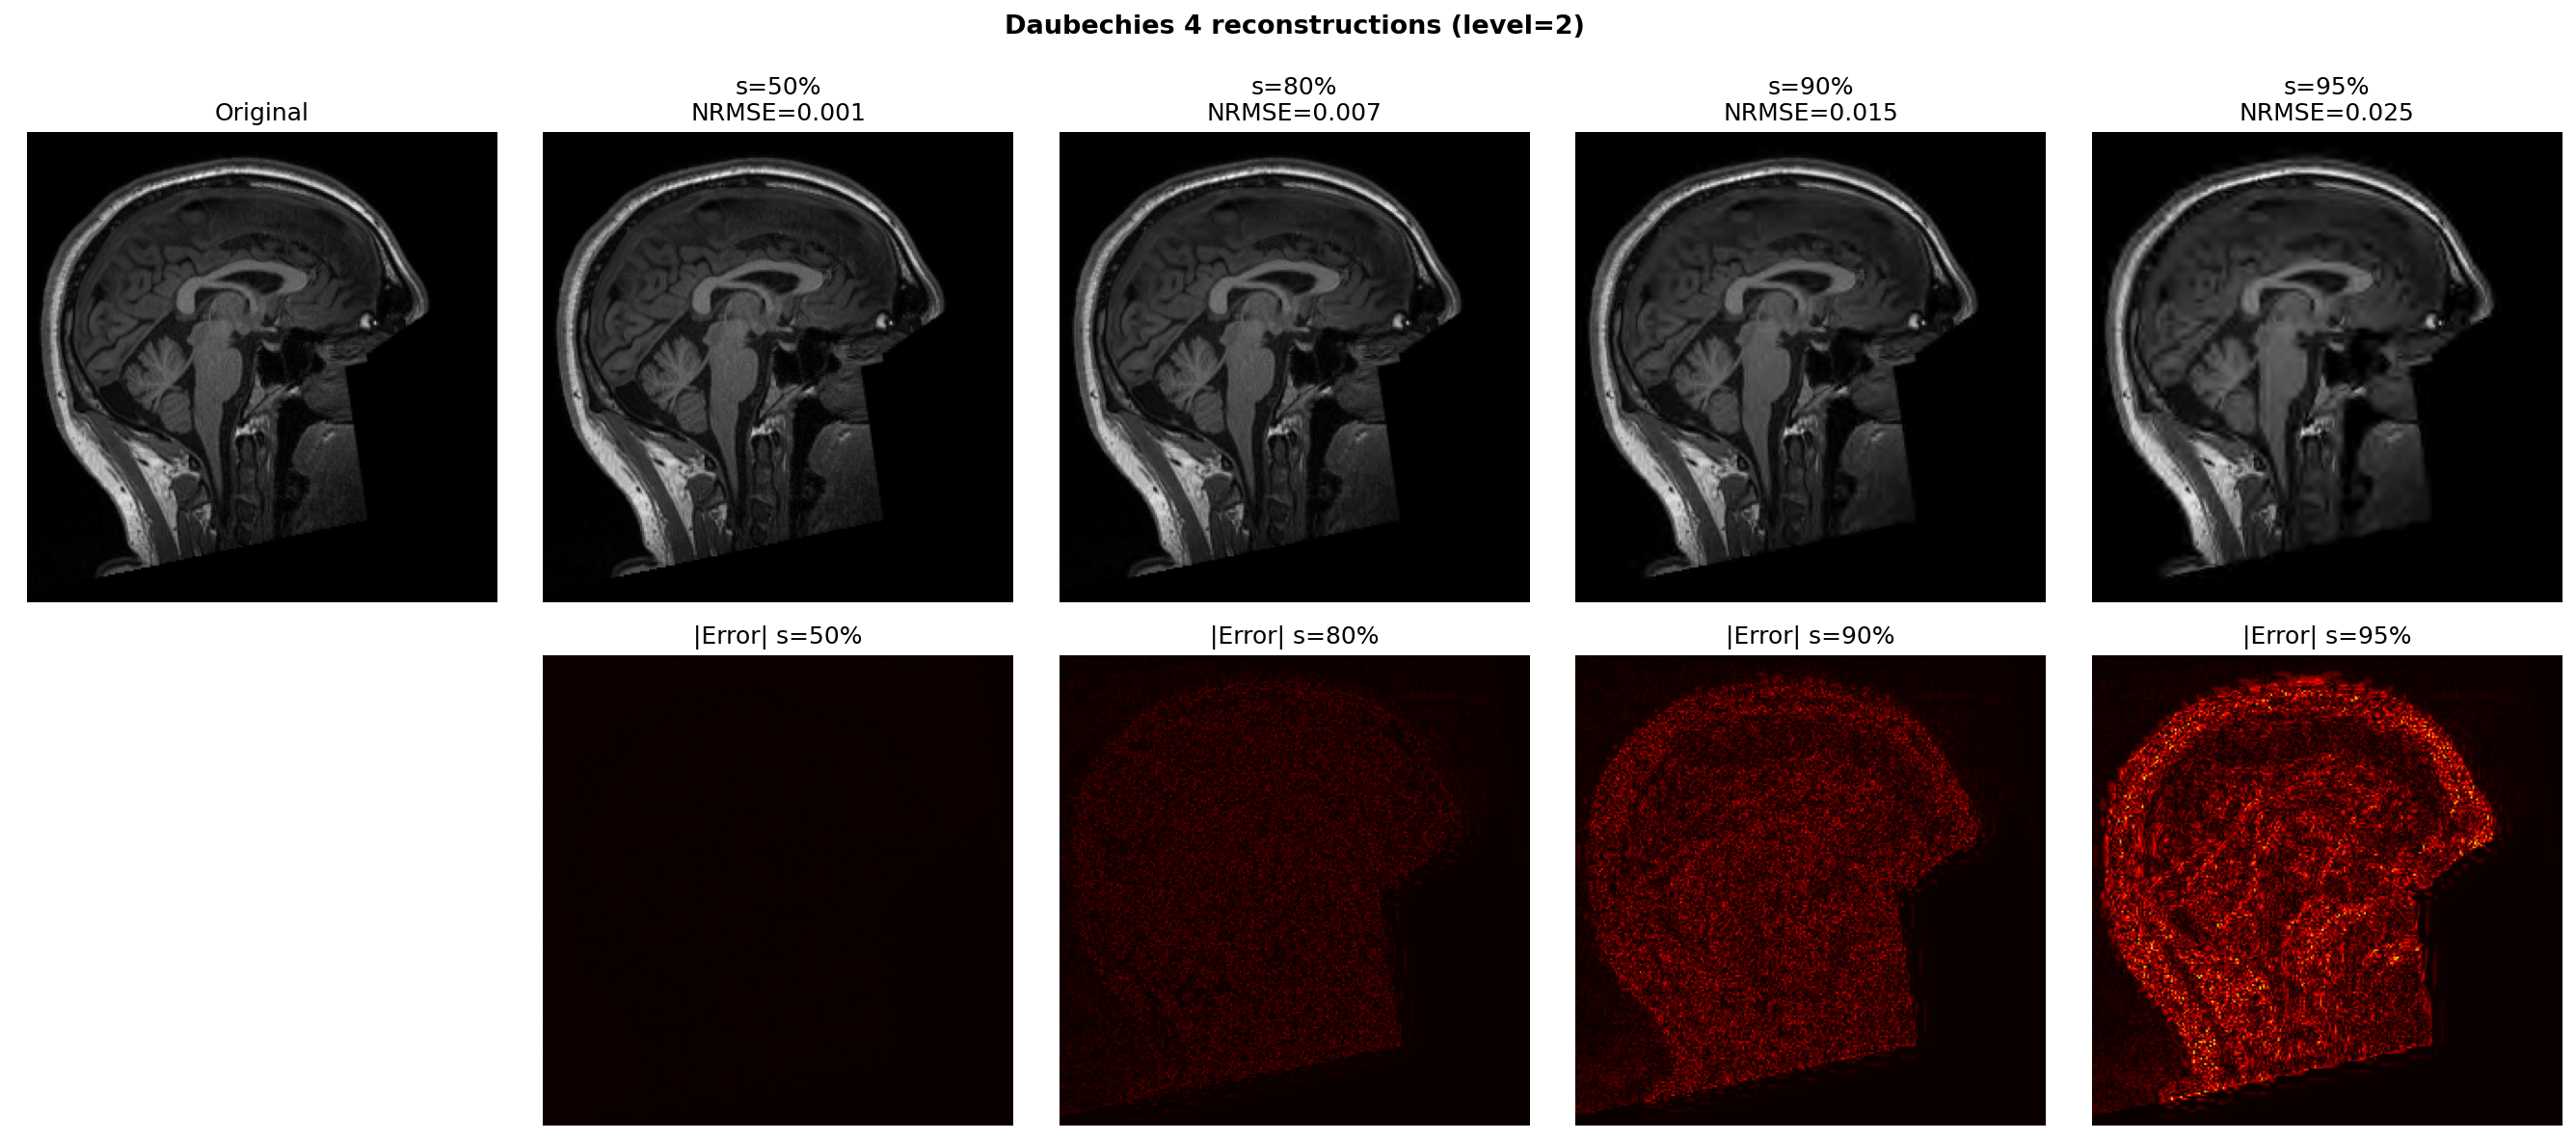
\includegraphics[width=0.9\linewidth]{Results/part5C_recons_db4.png}
  \caption{Daubechies~4 reconstructions at $s \in \{50, 80, 90, 95\}\%$
  (level=2). Top: reconstructed images. Bottom: absolute error maps.}
  \label{fig:recons_db4}
\end{figure}

\begin{figure}[h]
  \centering
  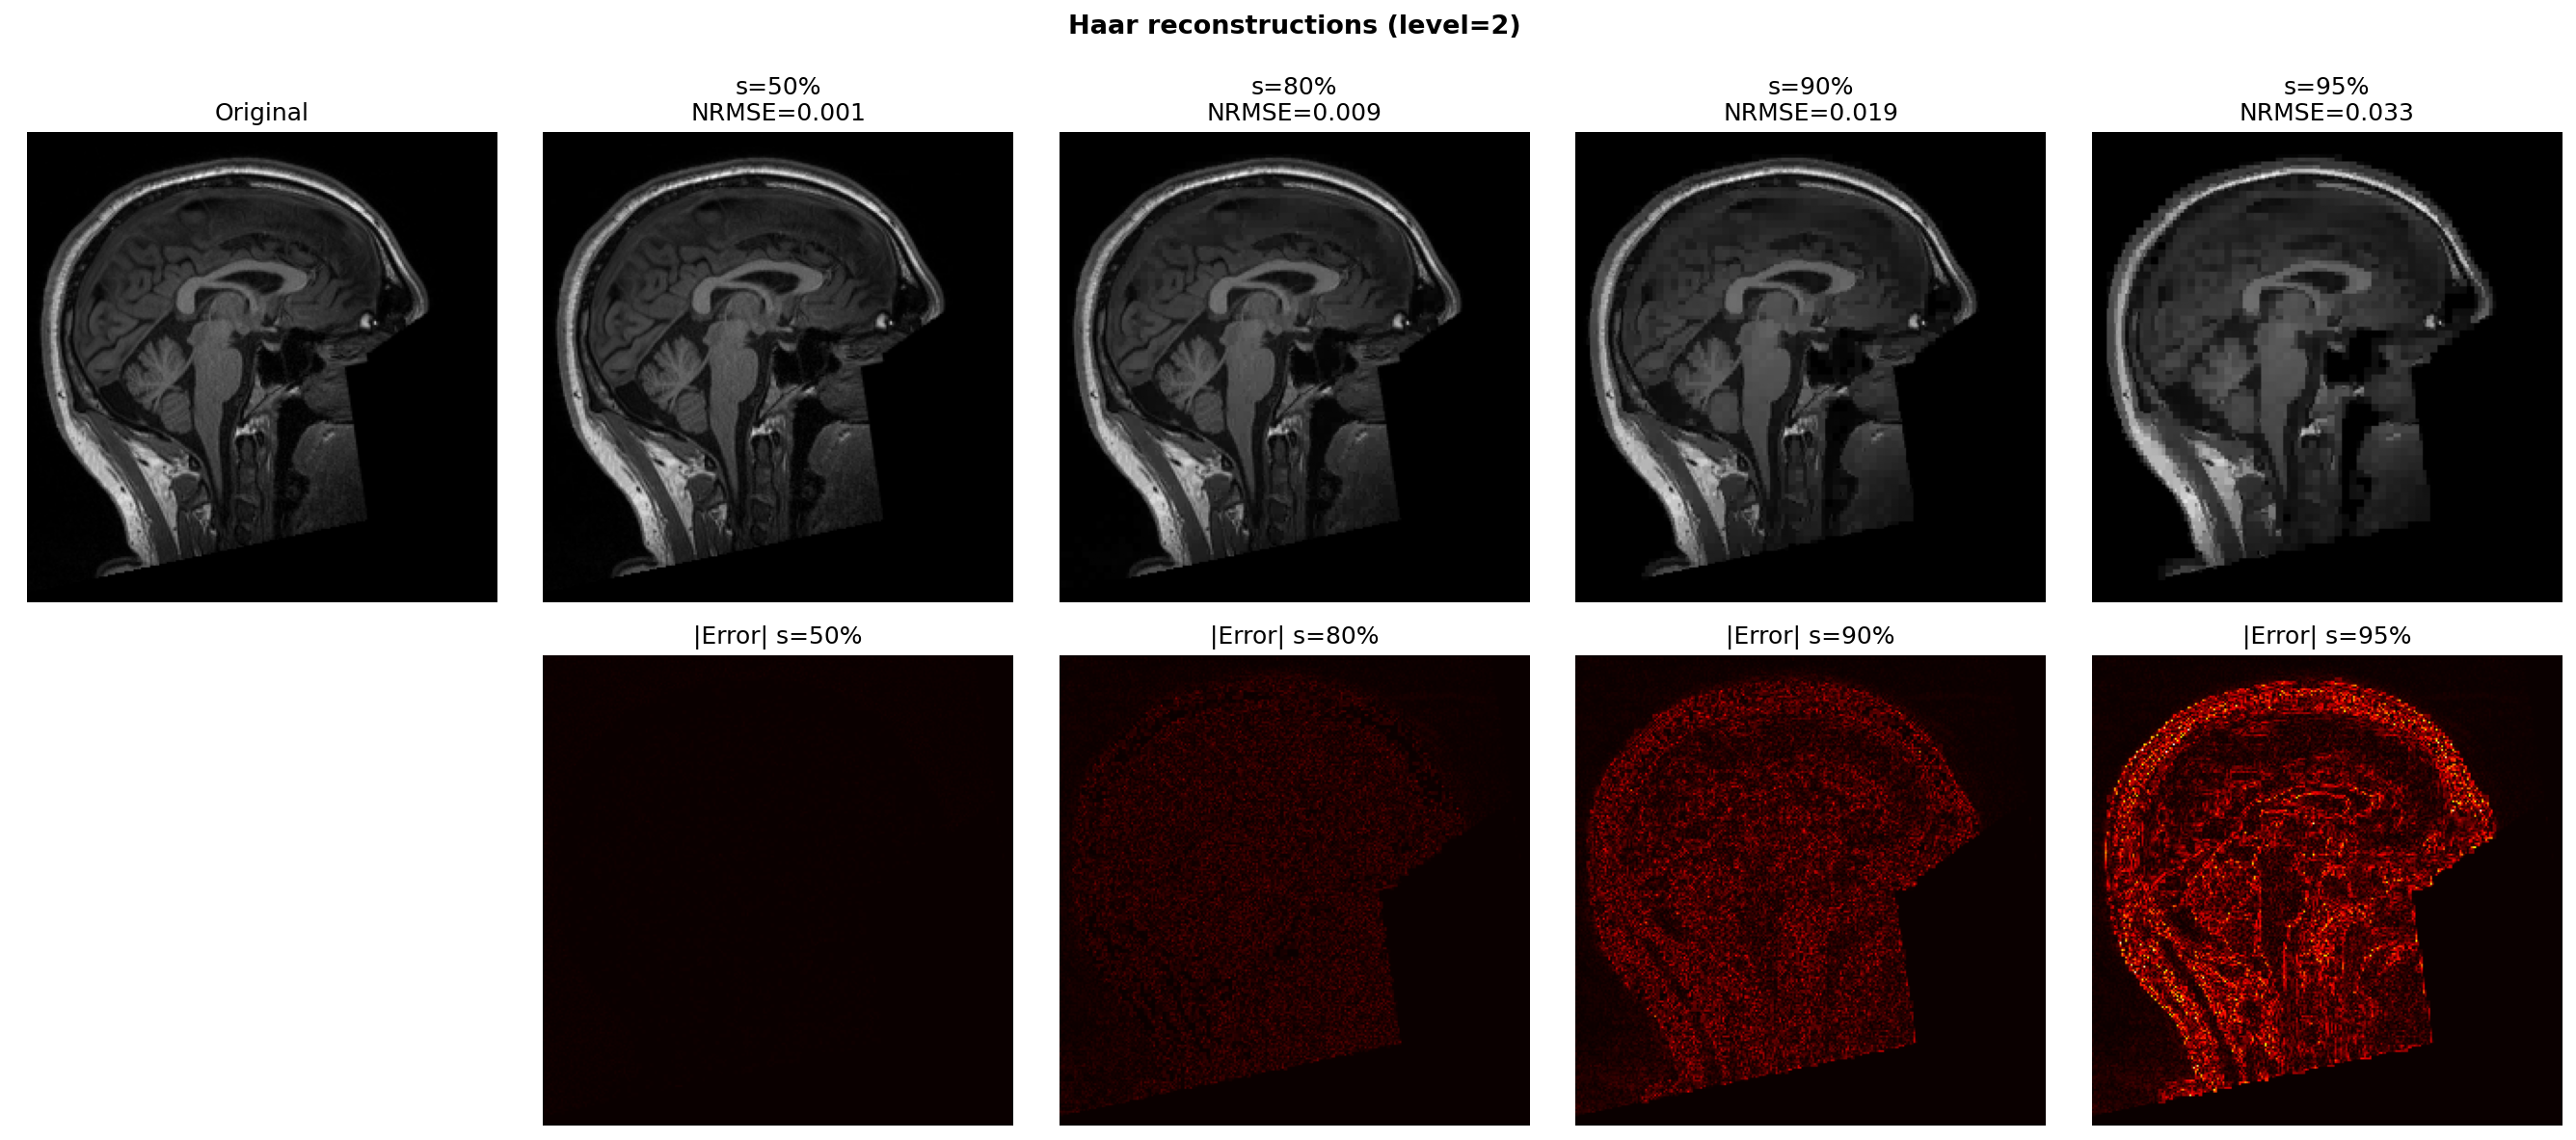
\includegraphics[width=0.9\linewidth]{Results/part5C_recons_haar.png}
  \caption{Haar reconstructions at $s \in \{50, 80, 90, 95\}\%$
  (level=2). Top: reconstructed images. Bottom: absolute error maps.}
  \label{fig:recons_haar}
\end{figure}
At $s=95\%$, Haar (NRMSE $= 0.033$) shows noticeably more
error than Daubechies~4 (0.025) and Coiflet~3 (0.022), consistent with
the sparsity ordering established in Section~\ref{sec:wavelet}.

Table~\ref{tab:threshold} states the minimum fraction of coefficients that
must be retained to keep NRMSE below 10\%.  At level~2, Daubechies~4 and
Coiflet~3 never cross the threshold; even discarding 99\% of coefficients
(retaining only 656 of 65,536) leaves NRMSE within acceptable bounds.  For
Haar at level~2, the boundary is crossed only at $s=99\%$.

\begin{table}[h]
\centering
\caption{Compression performance at the 10\% NRMSE boundary (level=2).}
\label{tab:threshold}
\begin{tabular}{lrr}
\toprule
Basis & $s^*$ & Coefficients kept \\
\midrule
Haar          & 99\%    & 655 / 65,536 \\
Daubechies~4  & $>$99\% & $\leq 656$   \\
Coiflet~3     & $>$99\% & $\leq 656$   \\
\bottomrule
\end{tabular}
\end{table}

We should note that at $s=80\%$, Coiflet~3 (level=2)
compression yields $\mathrm{NRMSE}=0.006$, whereas Fourier compression at
$s=50\%$ yields $\mathrm{NRMSE}=0.0087$ with severe 
artifacts.  The wavelet basis achieves substantially better compression for the same numerical "grade," underscoring the importance of human interpretability when deciding "how" to build a medical imaging pipeline.

\subsection{Effect of Decomposition Level}

Figure~\ref{fig:levels} shows Coiflet~3 reconstructions at $s=90\%$ for
decomposition levels 1, 2, and 3. Though not visually perceptible, Level~1 has the highest error (NRMSE $= 0.025$), while levels~2 and 3 both achieve NRMSE $=
0.013$.  Deeper decompositions push more energy into a
compact approximation subband, so the same threshold discards a larger
share of near-zero detail coefficients without removing structurally
important ones.

\begin{figure}[h]
  \centering
  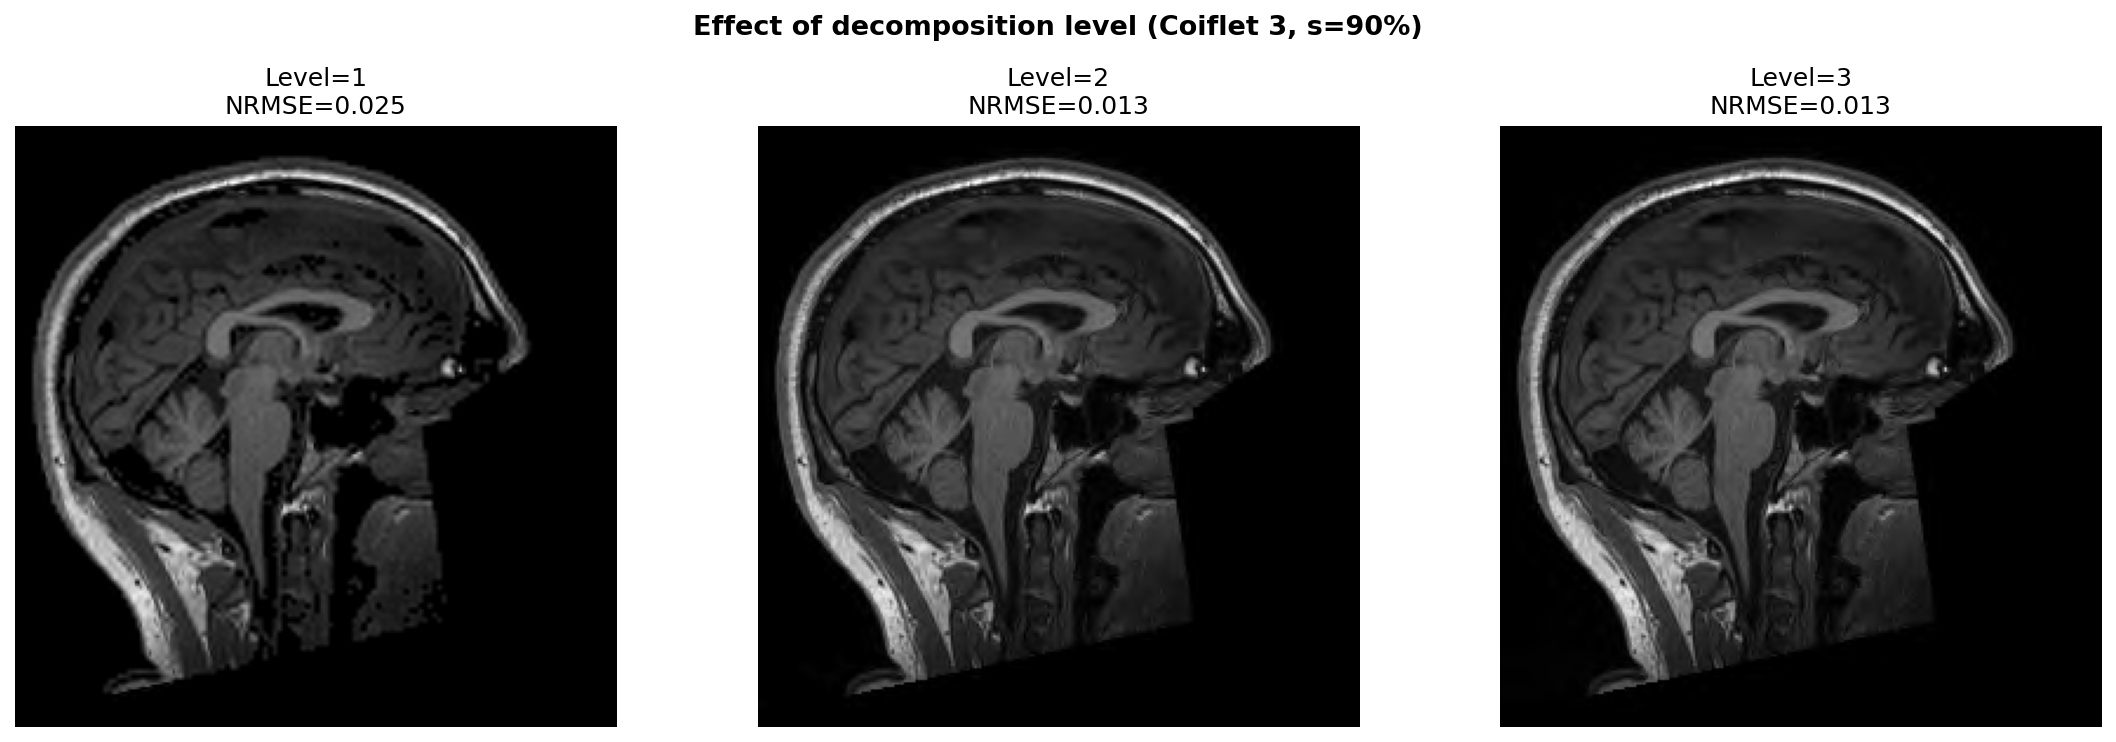
\includegraphics[width=0.9\linewidth]{Results/part5D_levels.png}
  \caption{Coiflet~3 reconstructions at $s=90\%$ for decomposition levels
  1, 2, and 3.}
  \label{fig:levels}
\end{figure}

\subsection{Generalization Across Slices and Contrasts}

Figure~\ref{fig:generalization} applies the same compression ($s=90\%$,
Coiflet~3, level=2) to four additional images: a T1 sagittal slice offset
from center, the T1 coronal and axial center slices, and the T2 sagittal
center slice.  NRMSE values of 0.013, 0.019, 0.018, and 0.016 respectively
are all comparable to the guiding image result, confirming that the sparsity
result holds across viewing planes and imaging contrasts.

\begin{figure}[h]
  \centering
  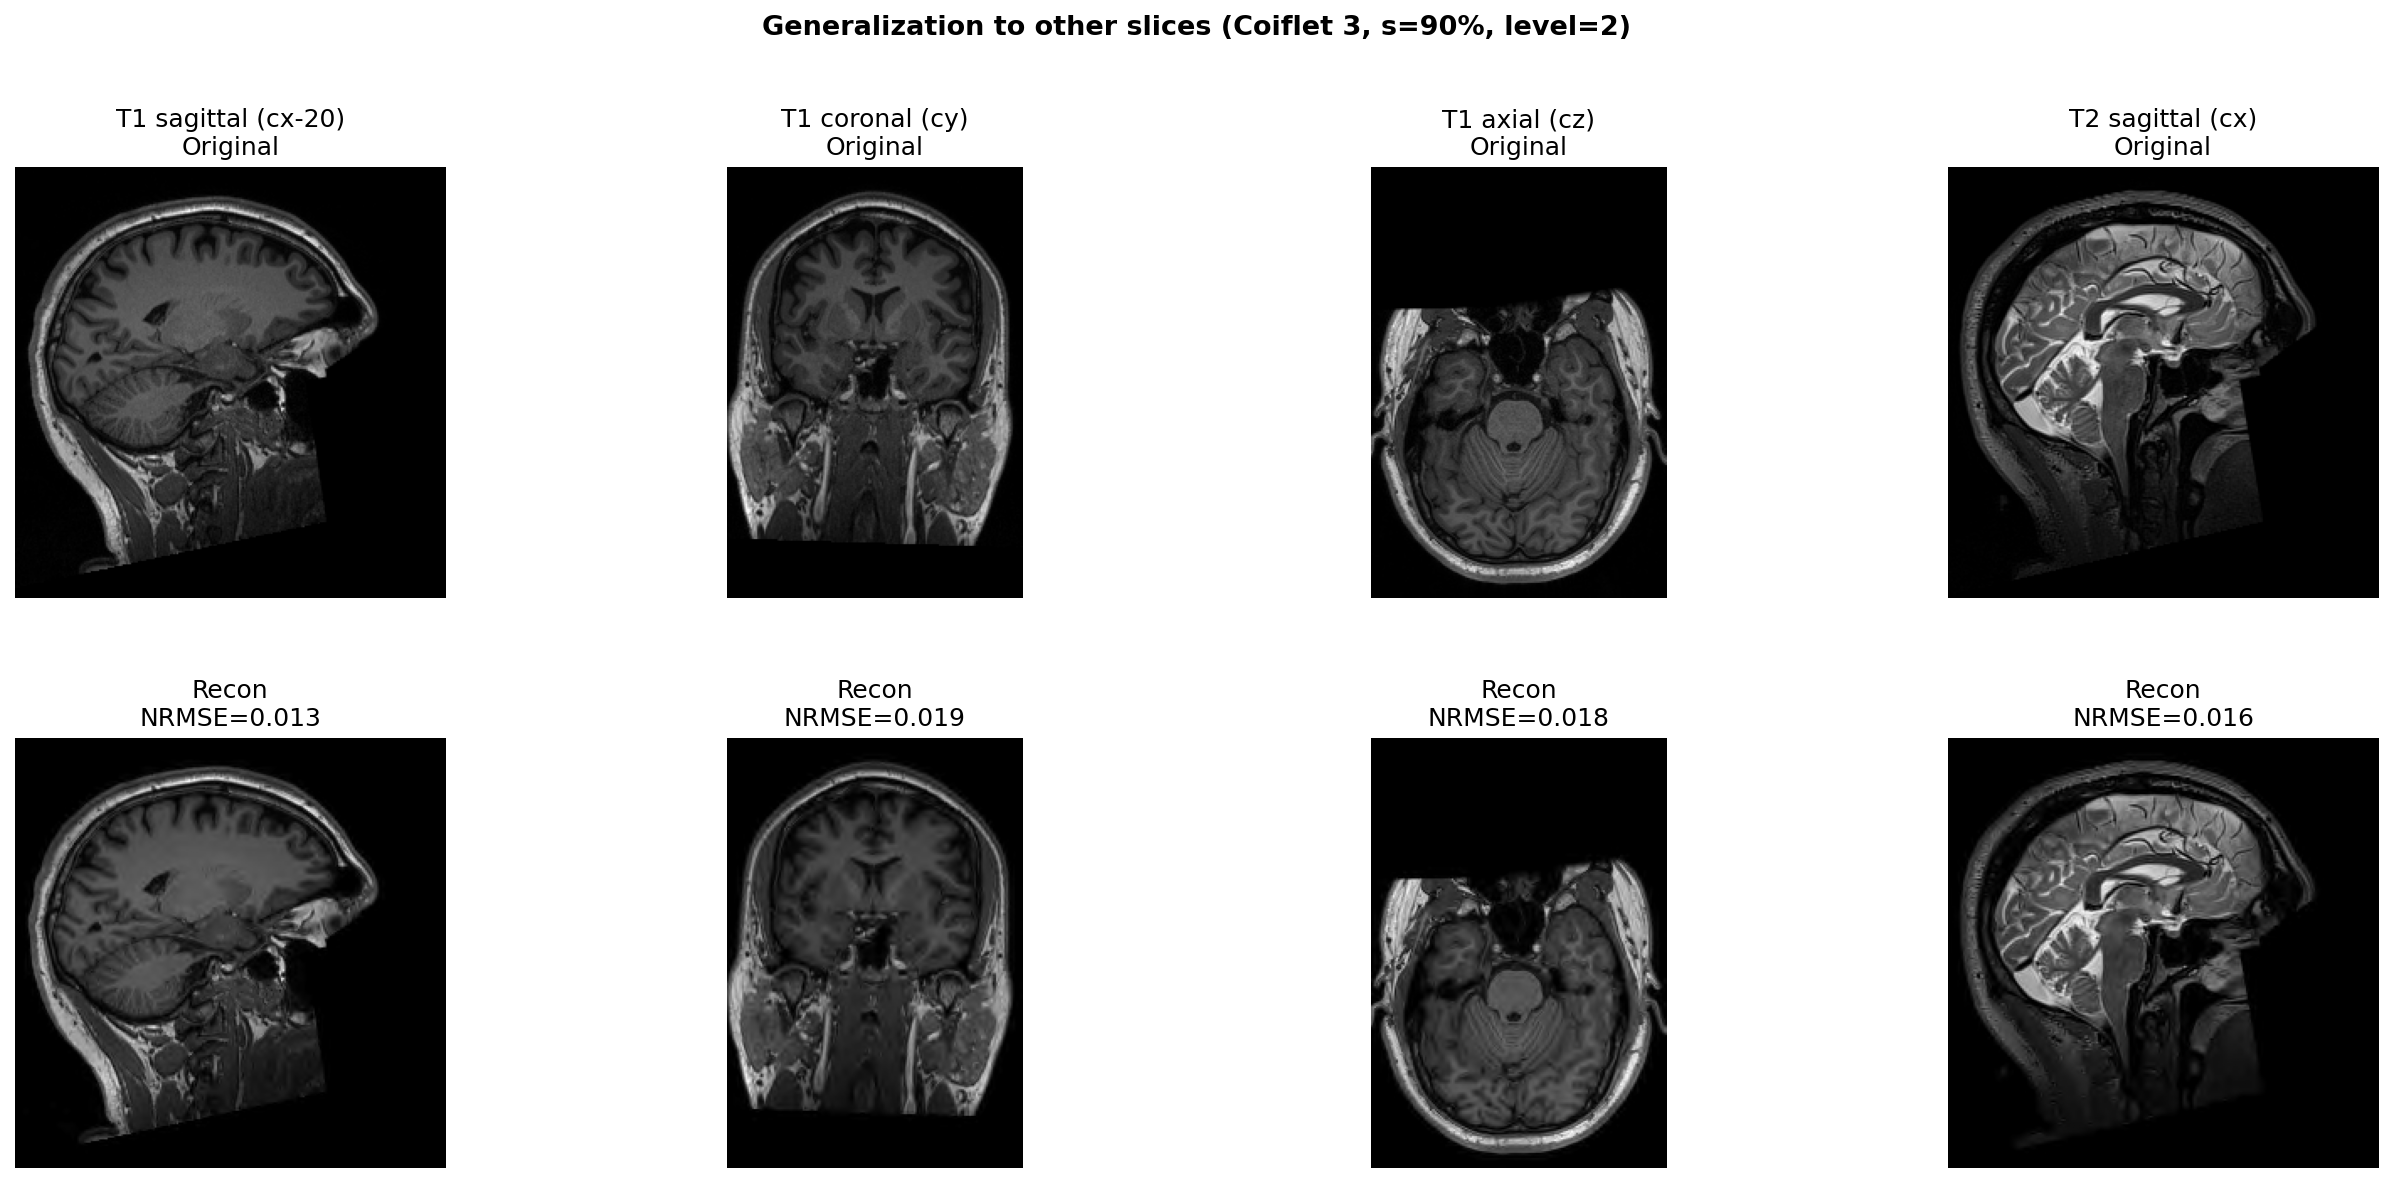
\includegraphics[width=0.9\linewidth]{Results/part5E_generalization.png}
  \caption{Coiflet~3 compression ($s=90\%$, level=2) applied to four
  additional slices. Top: originals. Bottom: reconstructions with NRMSE.}
  \label{fig:generalization}
\end{figure}

Figure~\ref{fig:per_slice} shows NRMSE at $s=99\%$ across all 176 T1
sagittal slices. Even the worst-case central slices, when they ocassionaly exceed the threshold, remain near the $10\%$ mark rather than far above it.


\begin{figure}[h]
  \centering
  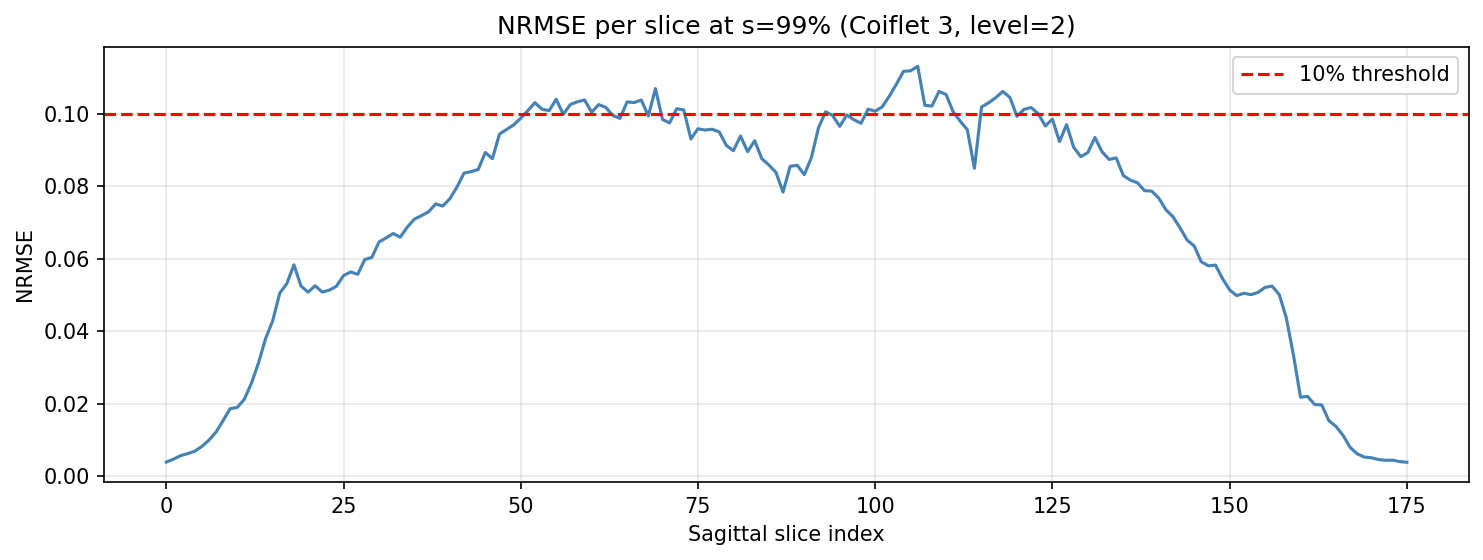
\includegraphics[width=0.9\linewidth]{Results/part5F_per_slice_error.png}
  \caption{NRMSE per sagittal slice at $s=99\%$ (Coiflet~3, level=2).
  Red dashed line: 10\% threshold.}
  \label{fig:per_slice}
\end{figure}

% ===========================================================================
\section{Compressed Sensing}
\label{sec:cs}

The CS experiments use the Coiflet~3 wavelet (level=2) as the sparsifying
basis, motivated by its superior compression performance established in
Section~\ref{sec:sparsity}.  The guiding image is normalized to $[0,1]$
before use.  Ground truth k-space is the 2D DFT of this normalized image,
which is then undersampled by a Bernoulli random mask with probability $p$.
ISTA (Algorithm~\ref{alg:ista}) recovers the image from the masked
measurements.


\subsection{Parameter Selection}
\label{sec:cs_params}

Figure~\ref{fig:lambda_eta_sweep} shows the ISTA objective over 200
iterations for all combinations of $\eta \in \{0.01, 0.1, 0.5, 0.75,
1.0\}$ and $\lambda \in \{10^{-4}, 10^{-3}, 5\times10^{-3}, 10^{-2}\}$
at $p=0.5$.  At $\eta=0.01$ the objective is still decreasing linearly at
200 iterations, so convergence is far too slow to be practical.  At
$\eta=0.1$ convergence is faster but the curves have not yet plateaued.
Both $\eta=0.5$ and $\eta=0.75$ converge cleanly by around iteration~75,
while $\eta=1.0$ shows a similar rate but with slightly less stable
behavior at early iterations.

\begin{figure}[h]
  \centering
  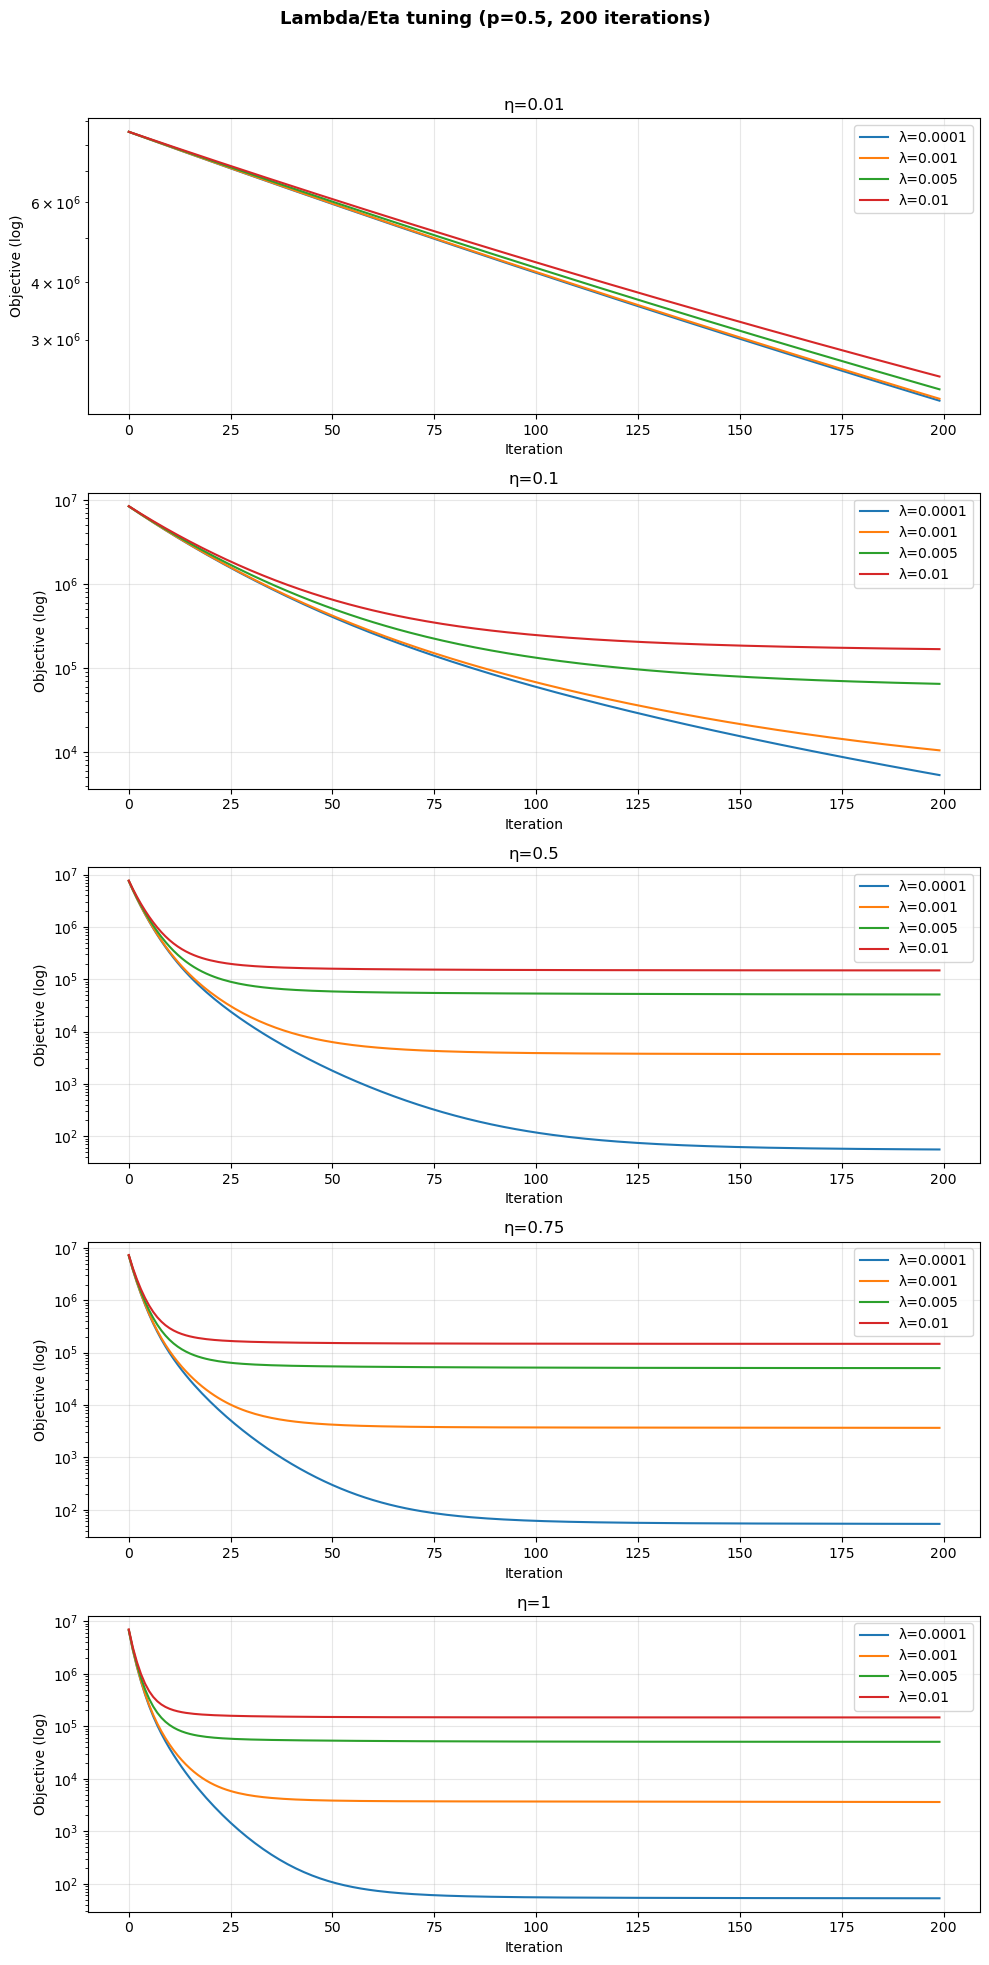
\includegraphics[width=0.65\linewidth]{Results/part6A_lambda_eta_sweep.png}
  \caption{ISTA objective vs.\ iteration for all $\eta$/$\lambda$
  combinations ($p=0.5$, 200 iterations, semilog scale).}
  \label{fig:lambda_eta_sweep}
\end{figure}

Figure~\ref{fig:quality_check} compares reconstruction quality for
$\eta \in \{0.5, 0.75\}$ and $\lambda \in \{10^{-4}, 10^{-3},
5\times10^{-3}\}$.  Smaller $\lambda$ under-regularizes, leaving residual
noise in the reconstruction; larger $\lambda$ over-smooths fine detail.
The combination $\eta=0.75$, $\lambda=0.005$ achieves the best NRMSE of
0.011 and is selected for all subsequent experiments.

\begin{figure}[h]
  \centering
  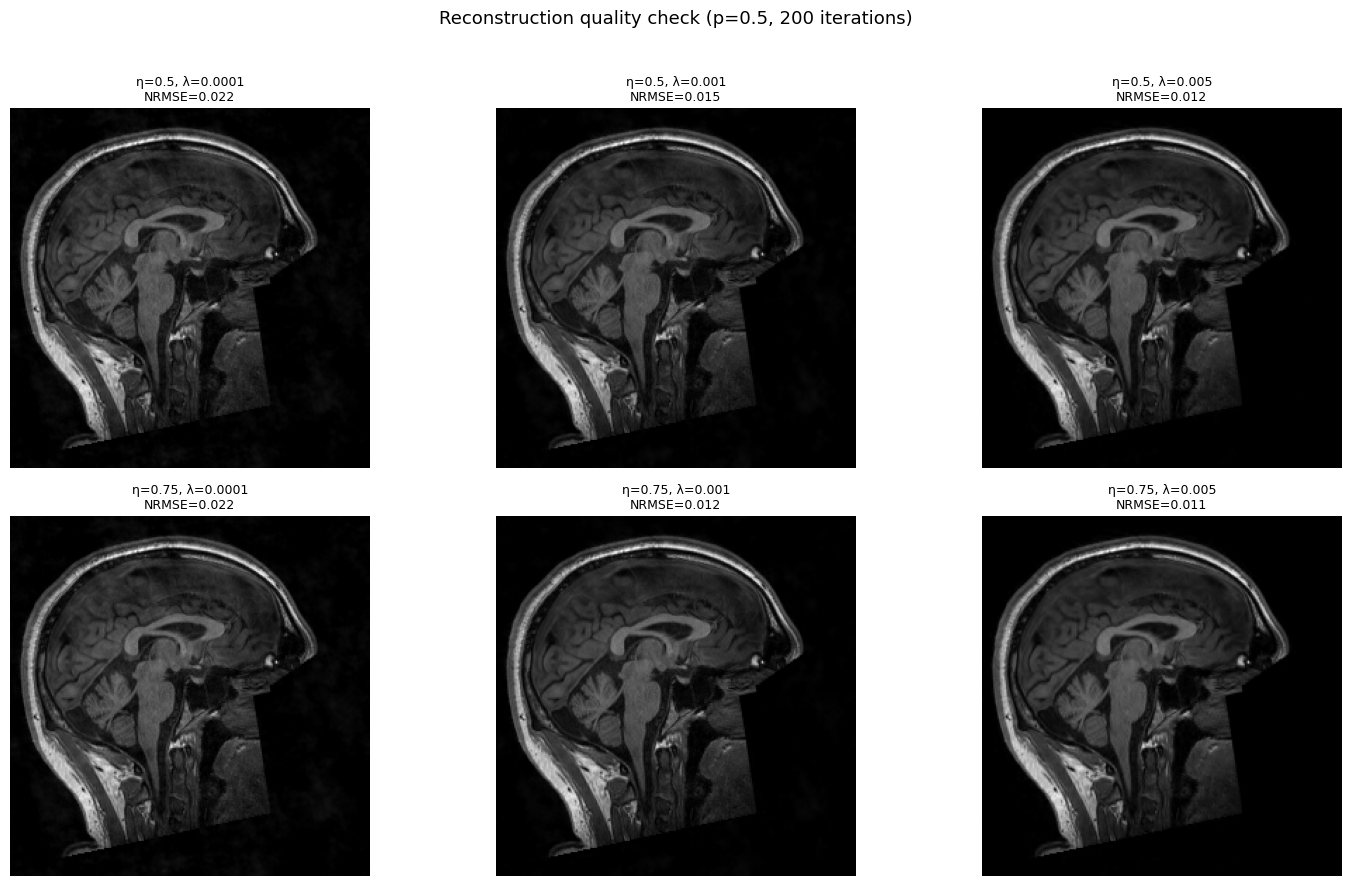
\includegraphics[width=0.9\linewidth]{Results/part6A_quality_check.png}
  \caption{Reconstructions at $p=0.5$, 200 iterations, for a subset of
  $\eta$/$\lambda$ combinations.}
  \label{fig:quality_check}
\end{figure}

\subsection{Convergence Analysis}

Figure~\ref{fig:convergence} shows the mean ISTA objective (averaged over
$N=1000$ random Bernoulli masks) as a function of iteration for
$p \in \{0.1, 0.25, 0.5, 0.75\}$.  All curves exhibit rapid initial descent
followed by a slower asymptotic plateau, visually seeming to follow a $1/k$ mode of decrease.  Higher $p$ values achieve lower final
objectives, as more k-space measurements constrain the solution more tightly.

\begin{figure}[h]
  \centering
  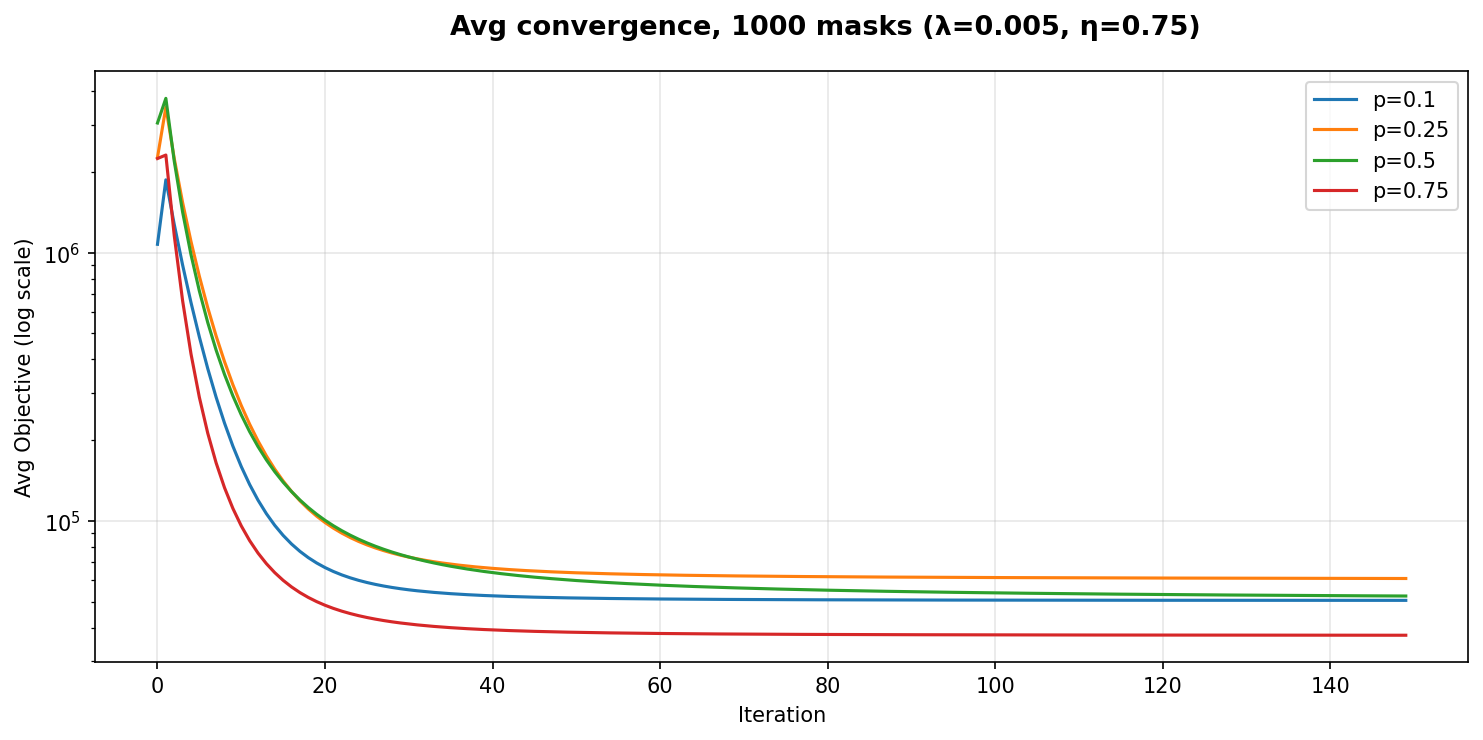
\includegraphics[width=0.9\linewidth]{Results/part6B_convergence.png}
  \caption{Mean ISTA objective vs.\ iteration for $p \in \{0.1, 0.25, 0.5,
  0.75\}$ averaged over $N=1000$ masks. Semilog scale.}
  \label{fig:convergence}
\end{figure}

\subsection{Reconstruction Quality vs.\ Sampling Fraction}

Figure~\ref{fig:cs_recons} shows reconstructed images and absolute error maps at each $p$ value.

\begin{figure}[h]
  \centering
  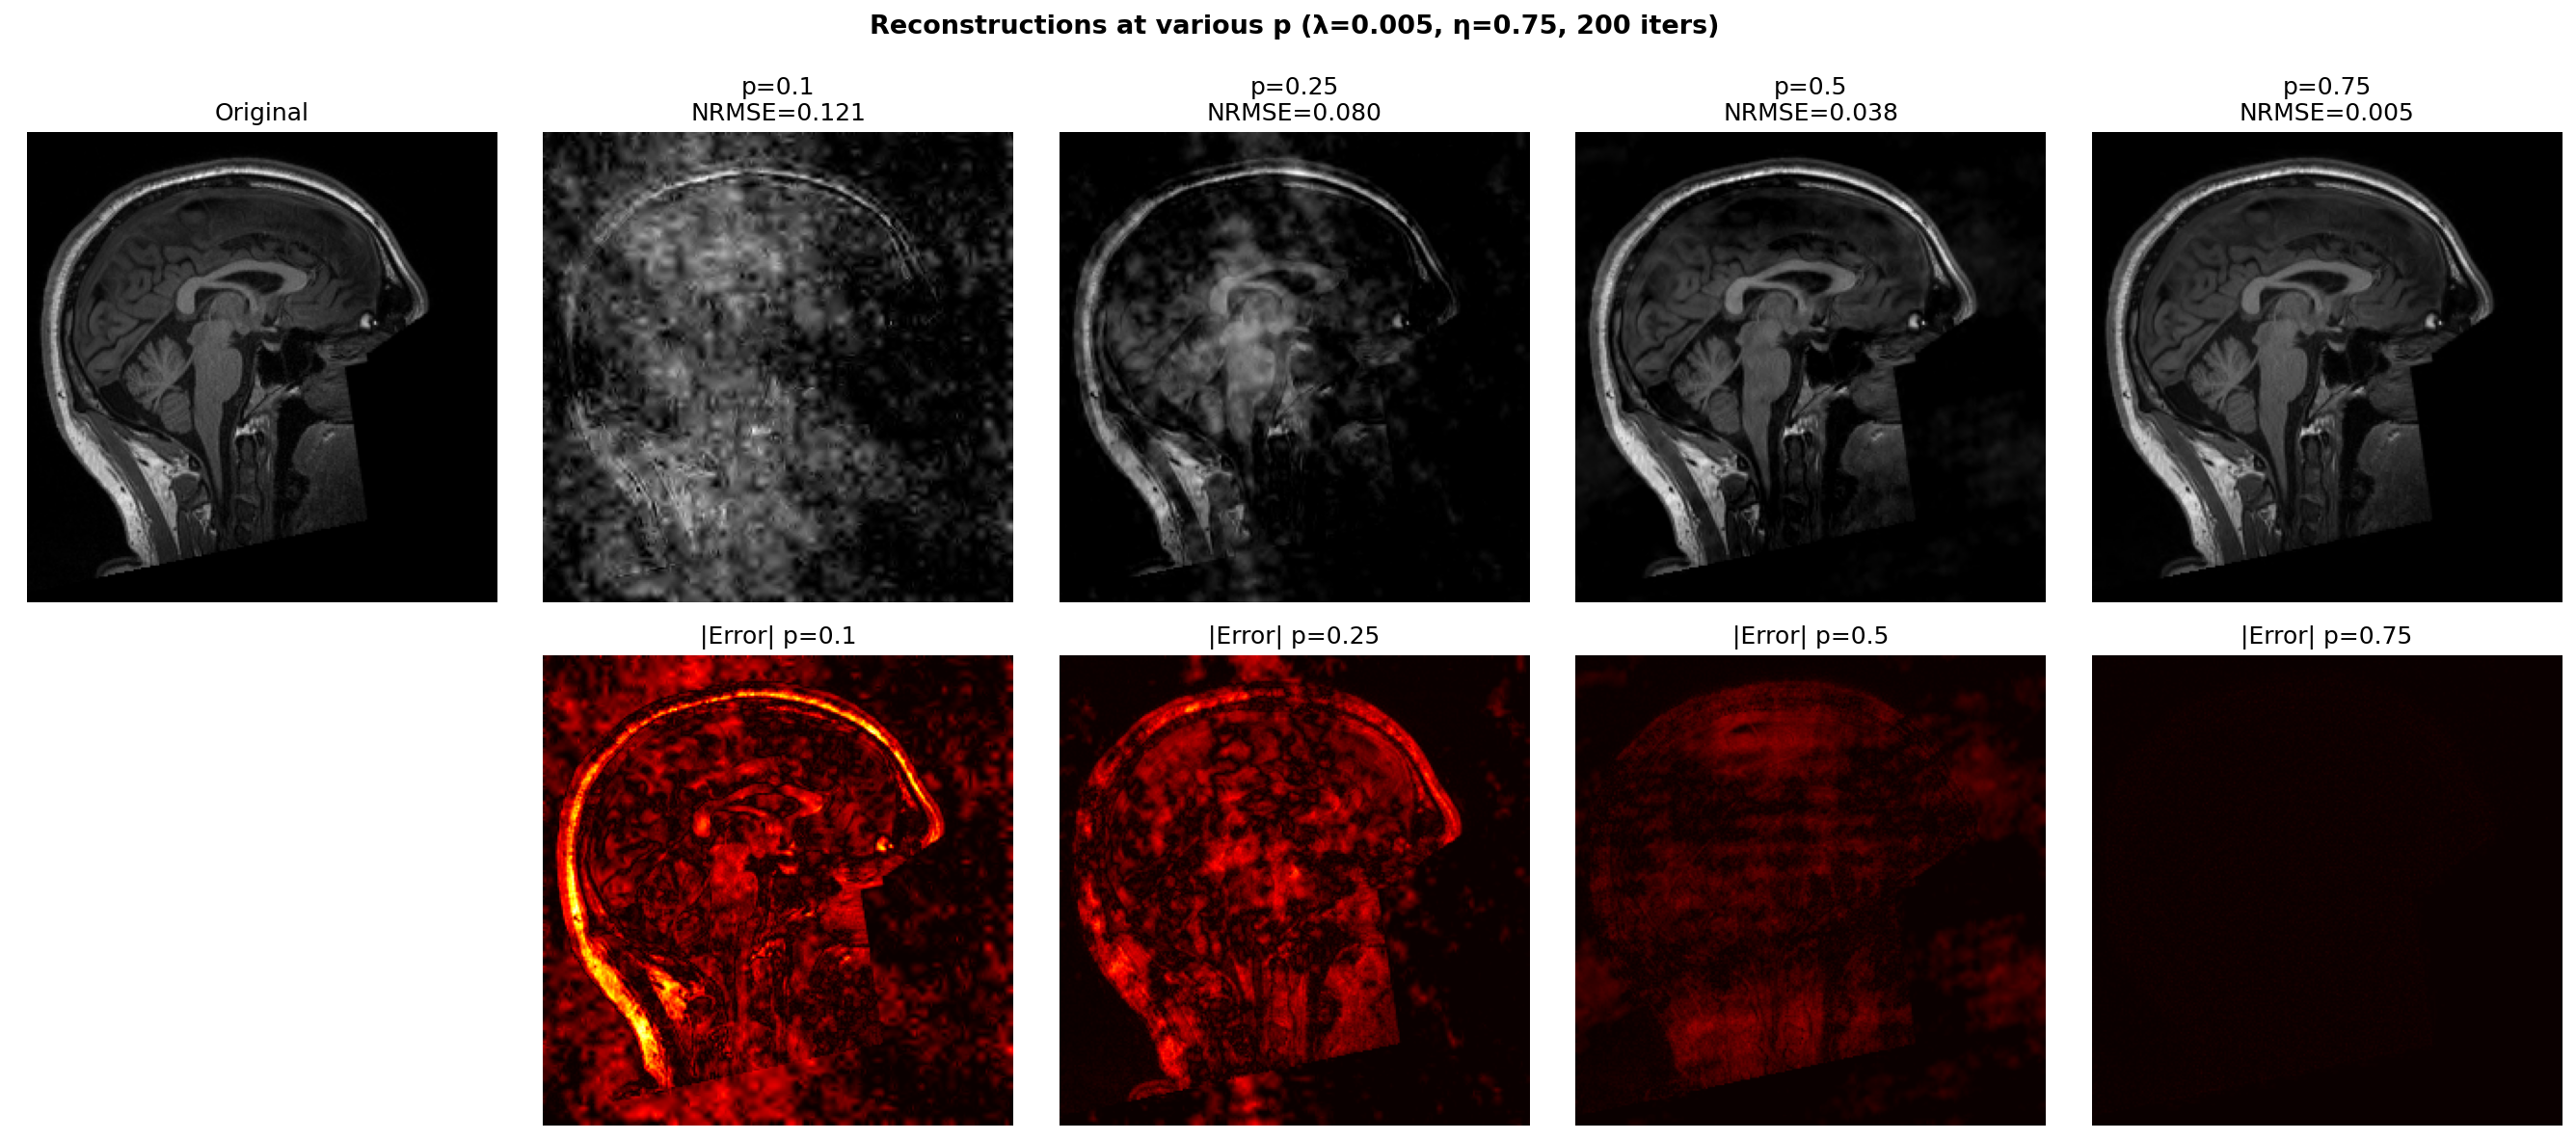
\includegraphics[width=0.9\linewidth]{Results/part6C_reconstructions.png}
  \caption{CS reconstructions at $p \in \{0.1, 0.25, 0.5, 0.75\}$
  ($\eta=0.75$, $\lambda=0.005$, 150 iterations).
  Top: reconstructed images. Bottom: absolute error maps.}
  \label{fig:cs_recons}
\end{figure}

At $p=0.75$ (NRMSE $= 0.005$), we get near-perfect anatomical recovery.  The error map is nearly black, with only faint residuals visible at the image boundary.

At $p=0.5$ (NRMSE $= 0.038$), the image still retains excellent visual quality.  All major anatomical structures are faithfully reconstructed.  This halves the scan time relative to full k-space coverage.

At $p=0.25$ (NRMSE $= 0.080$), the image appears substantially degraded.  The reconstruction is recognizable but exhibits patchy artifacts throughout that occlude the original image, and fine anatomical detail is lost.

At $p=0.1$ (NRMSE $= 0.121$), the image is severely degraded.  With only 10\% of k-space sampled, the reconstruction bears little resemblance to the original; the error map is bright across the entire image.

It appears in our trials that $p=0.5$ is the preferred operating point, reducing scan time by 50\% while maintaining NRMSE below 5\%.  Sampling at or below $p=0.25$ produces clinically unacceptable reconstructions for this image and specific CS setup.


% ===========================================================================
\section{Conclusion}
\label{sec:conclusion}

Through this work, we reached several main conclusions.

Fourier compression is fundamentally limited, as despite clear magnitude
sparsity in the Fourier domain, discarding low-magnitude coefficients
produces visually unacceptable images even when MSE appears small.  Phase
is globally coupled and non-redundant, and cannot be selectively discarded.

Wavelet compression, by contrast, succeeds.  The Coiflet~3 basis at
decomposition level~2 permits discarding over 99\% of coefficients while
maintaining NRMSE below 10\%, achieving a compression ratio exceeding
100:1 on a $256\times176$ image.  The choice of basis matters as well. As
anatomical brain images contain sharp edges and piecewise-smooth regions,
a basis with better space--frequency localization such as Coiflet~3
outperforms Daubechies~4 and Haar.  At a fixed compression ratio,
higher decomposition levels further concentrate energy into the
approximation subband, reducing the proportion of large detail
coefficients and lowering NRMSE.

Finally, ISTA-based CS can faithfully reconstruct MRI from intentionally
undersampled k-space.  With $\lambda=0.005$, $\eta=0.75$, and 150
iterations, Coiflet~3 wavelet sparsity yields NRMSE $\approx 3.8\%$ at
$p=0.5$, rising to $8.0\%$ at $p=0.25$ and severe degradation at
$p=0.1$.  This
demonstrates that the wavelet sparsity observed in Section~\ref{sec:sparsity} can be made clinically relevant, as real scan-time reductions (we saw up to $50\%$) are possible without
meaningful loss of diagnostic information.


Future directions include Total Variation (TV) and Total Generalized
Variation (TGV) regularization as alternative sparsity priors, 3D CS
operating on full volumes rather than 2D slices, and structured
undersampling patterns such as radial trajectories, which may improve incoherence and push the viable sampling fraction below $p=0.5$.

% ===========================================================================
\printbibliography

% ===========================================================================
\appendix
\counterwithin{figure}{section}
\counterwithin{table}{section}

\section{Auxiliary Functions}
\label{app:aux}

The following functions were defined in \texttt{aux\_functions.py} and reused
throughout the project.

\begin{description}
  \item[\texttt{scale\_magnitude(arr)}] Normalizes the input array to $[0,1]$
  by subtracting the minimum and dividing by the range.

  \item[\texttt{load\_volume(path)}] Loads a NIfTI file with \texttt{nibabel}
  and returns the array cast to \texttt{numpy.ndarray}.

  \item[\texttt{get\_center\_slices(vol)}] Returns $(c_x, c_y, c_z) =
  \lfloor\mathrm{shape}/2\rfloor$ for the three canonical planes.

  \item[\texttt{extract\_slices(vol, cx, cy, cz)}] Returns the triplet
  $[\mathbf{v}[c_x,:,:],\ \mathbf{v}[:,c_y,:],\ \mathbf{v}[:,:,c_z]]$.

  \item[\texttt{simple\_compression(arr, s)}] Zeros the lowest-magnitude
  $s$-th percentile of values in \texttt{arr}, returning an array of the same
  shape.

  \item[\texttt{mse(gt, recon)}] Computes $\frac{1}{N}\sum_i (x_i -
  \hat{x}_i)^2$ on raw pixel values.

  \item[\texttt{nrmse(gt, recon)}] Computes $\sqrt{\mathrm{MSE}}/\max(\mathbf{x})$,
  the primary scalar error metric used throughout this report.

  \item[\texttt{plot\_wavelet(image, wavelet, level)}] Computes a 2D DWT and displays the approximation subband and all detail subbands in a single multi-panel figure.
\end{description}

\section{ISTA Implementation Notes}
\label{app:ista}

The forward operator $\mathcal{M}(\boldsymbol{\omega})$ is implemented as:
\begin{enumerate}
  \item Reconstruct the spatial image $\hat{\mathbf{x}} =
  \boldsymbol{\Psi}^{-1}\boldsymbol{\omega}$ via \texttt{waverec2}, cropped
  to $H\times W$.
  \item Apply 2D DFT via \texttt{numpy.fft.fft2}.
  \item Element-wise multiply by the binary mask $\mathbf{M}$.
\end{enumerate}

The adjoint $\mathcal{M}^*(\mathbf{v})$ is:
\begin{enumerate}
  \item Element-wise multiply by $\mathbf{M}$ (zero-fill unobserved
  frequencies).
  \item Apply inverse DFT and take the real part.
  \item Apply DWT via \texttt{wavedec2} and flatten coefficients.
\end{enumerate}

The objective loss is recorded \emph{before} renormalization each iteration
using the already-computed Fourier residual, so it correctly reflects the
$\ell_2$ fidelity term without the clipping nonlinearity.

\end{document}